\label{sec:design}
The design combines a Cartesian pen plotter with three processing stages: page conditioning and line segmentation, text and writer classification, and handwriting reproduction. The hardware is described first because its workspace, pen mechanism and achievable motion determine what the processing stages must produce. The software is then followed from a photographed page to a new piece of writing, before the complete operating sequence is described.

Implementation-specific equations, parameter values and pseudocode describe the project's CleanPipeline3 source~\cite{braunepipeline2026}; borrowed methods are cited at their point of use. Worked numerical examples are derived here unless identified as recorded measurements.\par

\subsection{Design summary}
\label{sec:des-summary}
This section summarises the project design tasks and how they were implemented (see Table~\ref{tab:des-summary}). The tasks follow the deliverables and student design work in the approved Project Proposal. Completion refers to the implementation of a task; compliance with a numerical system specification is established separately by the qualification tests in the Results section.

\begin{table}[!htbp]
\centering\small
\begin{tabularx}{\linewidth}{|>{\raggedright\arraybackslash}p{0.24\linewidth}|>{\raggedright\arraybackslash}X|>{\raggedright\arraybackslash}p{0.23\linewidth}|}
\hline
\textbf{Deliverable or task}&\textbf{Implementation}&\textbf{Completion of deliverable or task, and section in the report}\\\hline
Page capture and image conditioning&Camera arrangement, illumination normalisation, ink extraction and orientation correction.&Completed; Sections~\ref{sec:des-camera} and~\ref{sec:des-seg}.\\\hline
Separation of handwritten text&Line detection, curved separation boundaries and ink ownership produce recogniser inputs. Character localisation is performed later using known text.&Completed; Sections~\ref{sec:des-seg} and~\ref{sec:des-alignment}.\\\hline
Text and writer classifiers&Convolutional feature extraction, sequence recognition and a separate writer-identification head.&Completed; Section~\ref{sec:des-class}.\\\hline
Network training and verification&Numerical training implementation and a corresponding framework implementation; labelled public and personal handwriting data.&Completed; Sections~\ref{sec:des-training}--\ref{sec:des-netverify}.\\\hline
Writer-specific trajectory maps and storage&Aligned glyph extraction, skeleton tracing, variant filtering and persistent style profiles.&Completed; Sections~\ref{sec:des-alignment}--\ref{sec:des-profile}.\\\hline
Handwriting synthesis and G-code&Text layout, glyph assembly, candidate selection and conversion to machine coordinates.&Completed; Sections~\ref{sec:des-layout}--\ref{sec:des-gcode}.\\\hline
Gantry, pen mechanism and motion control&Custom mechanical assembly, two-axis drive, pen switching, end stops and calibration.&Completed; Section~\ref{sec:des-hardware}.\\\hline
Display and system communication&Web interface and server connect camera acquisition, classification, generation and physical writing.&Completed; Section~\ref{sec:des-integration}.\\\hline
\end{tabularx}
\caption{Design summary.}
\label{tab:des-summary}
\end{table}

The final implementation separates text into lines rather than requiring isolated letters before recognition. This allows connected handwriting to be read without committing to uncertain character boundaries. Character positions are recovered with known transcripts when constructing the glyph library. The text reader and writer classifier also use separate output heads because identifying a sequence of characters and identifying the writer require different treatment of position within a line. These choices retain the proposal's intended functions while changing how those functions are implemented.
\designgap{Confirm the completion entries against the final submitted deliverables, and identify the computer used for training and profile construction. The proposal's embedded-processing requirement must remain distinguishable from the actual training arrangement.}
\FloatBarrier

\subsection{System block diagram}
\label{sec:des-system}
The complete system has a physical interface and a processing interface. The camera supplies an image to the ODROID N2+, while the gantry receives motion commands from the same computer. Between these interfaces, line images, recognised strings, writer probabilities and pen trajectories are kept as different representations. This makes it possible to inspect the output of one stage before it is used by the next.

Figure~\ref{fig:des-hardware-system} shows the hardware connections. The two stepper drivers supply the winding currents; the ODROID supplies STEP and DIR signals rather than motor power through its GPIO pins. Four switches indicate the axis limits and a fifth indicates the pen state. The pen motor is controlled through its own switching circuit. Camera acquisition, inference and job execution are coordinated by the server.
\begin{figure}[!htbp]\centering
\designasset{design-hardware-overview.pdf}{0.96}{Labelled system diagram distinguishing motor power, logic signals, switch feedback and camera data.}
\caption{Hardware architecture of the handwriting robot.}
\label{fig:des-hardware-system}
\end{figure}

Figure~\ref{fig:des-processing-system} separates the three operating modes. During preparation, labelled line images train the text and writer models, and the text model is also used to extract a writer's glyphs from lines with known transcripts. The resulting weights and style profiles are stored for later use. During classification, the input page is conditioned and separated into lines; the reader produces text and the writer classifier produces a probability distribution over the trained writers. During reproduction, digital text and a selected profile are converted into a trajectory, then G-code, and finally GPIO pulses and pen commands.
\begin{figure}[!htbp]\centering
\designasset{design-processing-overview.pdf}{0.96}{Three paths: labelled pages to models/profiles; photographed page to text and writer; text plus selected profile to trajectory, G-code and gantry. Show stored artefacts and shared modules.}
\caption{Processing architecture and the stored information shared by the operating modes.}
\label{fig:des-processing-system}
\end{figure}

Recognition and reproduction share models, but they do not perform the same operation. Recognition estimates unknown text from an image. Glyph extraction uses text that is already known to estimate where its characters occur. Reproduction arranges the extracted pen paths into new text and uses the reader and writer classifier to select among candidate renderings. Keeping these roles separate is important: a candidate-selection score indicates how a model judges the generated image, whereas an independently assessed physical page establishes what the complete machine actually reproduced.

The interface between software and mechanics is G-code. It describes motion in millimetres and pen state without requiring the synthesiser to know GPIO pin numbers. Conversely, the motion interpreter can draw a geometric test file without loading a handwriting model. This separation supports commissioning the gantry independently and localising errors to image processing, trajectory generation or physical execution.
\FloatBarrier

\subsection{Hardware design}
\label{sec:des-hardware}
The hardware must hold the paper and pen securely, reach the required writing area, and convert a stored trajectory into repeatable motion. The design therefore combines a Cartesian belt drive with a separately actuated pen mechanism. The electrical interface is kept simple enough for direct control from the ODROID, while calibration relates software coordinates to the travel of the assembled machine.

\subsubsection{Plotter mechanics and mechanical construction}
The chosen method of text plotting is a Cartesian gantry system with two independent axes of movement and a pen up/down mechanism, consistent with the Cartesian arrangement illustrated by Teikari~\cite[p.~6, Fig.~4]{teikari2016}. Complex kinematic equations and joint-dependent position errors are avoided by using separate $x$ and $y$ movements for reproduction. Linear GT2 timing belts and pulleys are used to convert rotary motion from stepper motors and axles to the desired Cartesian movements. Timing belts were chosen for their cost effectiveness and ability to provide relatively fast travel without a lead-screw transmission.

A Cartesian gantry consists of stationary rails that guide movement in one axis, and a movable rail that guides the other axis of movement. For this system and the explanations that follow, the stationary rails guide $y$-axis movement, while the $x$-axis rail moves along the $y$-axis. Figure~\ref{fig:des-gantry-axes} shows the axes of the gantry.
\begin{figure}[!htbp]\centering
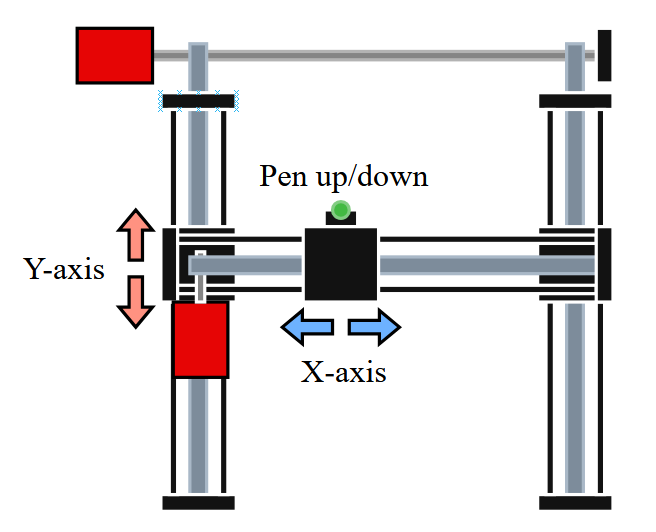
\includegraphics[width=0.67\linewidth]{Figures/gantry-axis-diagram.png}
\caption{Cartesian gantry axes and pen up/down mechanism.}
\label{fig:des-gantry-axes}
\end{figure}

The $x$-axis rail needs to move with stability and consistency, which is why it is supported at both ends by the two $y$-axis rails. A single stepper motor was chosen to drive the pulleys on both sides to ensure synchronised motion and save costs. Two independent stepper motors driving one axis introduce a synchronisation concern because differences in missed steps or loading could offset one side relative to the other. The challenge with using one motor to drive two timing pulleys is extending its shaft to both pulleys without excessive load or twist in the new axle. A rigid coupler was used to extend the stepper motor shaft with a chromed steel rod.

To reduce strain on the motors and allow smoother movement, linear bearings were fitted around the chromed rod rails so that the moving parts slide with low resistance. Bearing alignment is important as well as bearing diameter: an incorrectly aligned bearing can constrain the same rod in a different direction from the neighbouring bearing, increasing resistance instead of reducing it. During assembly, bearing fit and printed-part alignment were checked by sliding the parts along the rods before connecting the belts. The fit was adjusted where the assembled bearings restricted movement.

The shared shaft couples the two sides mechanically, but does not remove all sources of error. Unequal belt tension, shaft torsion and a frame that is not square can still change the pen position. Belt tension must therefore be sufficient to maintain engagement without adding unnecessary bearing load. The pen holder also needs enough stiffness to prevent lateral deflection as the direction of travel changes. These effects concern physical accuracy and cannot be inferred from the nominal step resolution alone.

The printed components locate bearings, support the motors and pulleys, fasten the belts, and guide the pen mechanism. Their relationship within the completed assembly is identified in Figure~\ref{fig:des-assembly}. The arrangement fixes the relative positions of the rail, belt and pen, so manufacturing fit and bracket stiffness affect the same position budget as the drive. The available travel is established in Section~\ref{sec:des-calibration}.
\begin{figure}[!htbp]\centering
\designasset{design-gantry-assembly.jpg}{0.85}{Photograph or assembled CAD view with the custom brackets, cross-shaft, belt tensioning, rail bearings and paper restraint labelled.}
\caption{Mechanical assembly and the components locating the pen relative to the page.}
\label{fig:des-assembly}
\end{figure}

\subsubsection{Stepper motor selection and drive resolution}
\label{sec:des-drive}
A stepper motor turns through fixed angular increments as the winding-current pattern changes. The windings are the motor's coils, and each current pattern establishes a magnetic field that pulls the rotor towards a corresponding position. The A4988 regulates these winding currents by chopping: it switches the drive to maintain the requested current level. Chopping continues even while a position is held; advancing the requested current pattern, rather than chopping itself, produces the next step~\cite[p.~9]{a4988ds}.

Two stepper motors are used in the gantry plotter, one for the $x$ and one for the $y$ direction. The selected motor is the 42BYGH40-01 NEMA 17 bipolar stepper, with a 40\,mm body length, a $1.8^\circ$ full-step angle and a rated current of 1.68\,A per phase. Stepper control suits the required position commands because displacement follows from the number of commanded steps, without requiring an encoder for normal operation. The corresponding limitation is that the controller cannot determine whether every commanded step was physically completed.

For the 20-tooth GT2 pulleys and 2\,mm belt pitch, the travel per revolution and pitch radius follow from Equation~\ref{eq:des-pulley}. The radius is determined by tooth pitch, rather than by measuring the shaft or outside pulley diameter.
\begin{equation}
\ell_{\mathrm{rev}}=N_t p=20(2)=40\ \mathrm{mm/rev},\qquad
r_p=\frac{N_t p}{2\pi}=6.37\ \mathrm{mm}.
\label{eq:des-pulley}
\end{equation}
Here $N_t$ is the tooth count and $p$ is belt pitch. With 200 full steps per revolution and a microstep subdivision $\mu_s=16$, the nominal commanded displacement is given by Equation~\ref{eq:des-stepres}.
\begin{equation}
\kappa_0=\frac{200\mu_s}{\ell_{\mathrm{rev}}}=80\ \mathrm{microsteps/mm},\qquad
\Delta x_0=\frac{1}{\kappa_0}=0.0125\ \mathrm{mm}.
\label{eq:des-stepres}
\end{equation}
The A4988 supports this subdivision through its microstep-selection inputs~\cite[p.~6, Table~1]{a4988ds}. The value in Equation~\ref{eq:des-stepres} is substantially smaller than the proposal's 0.5\,mm positional-error limit. It establishes adequate command granularity, but is not a measurement of accuracy: belt compliance, frame geometry, switch behaviour and pen deflection remain between the step count and the mark on paper. Microstepping also does not guarantee that every intermediate mechanical position is equally accurate under load.

Motor torque must be assessed at operating speed, rather than from holding torque alone. With feed $F$ in mm/min, Equation~\ref{eq:des-rpm} gives the motor speed. A travel feed of 4000\,mm/min corresponds to 100\,rev/min.
\begin{equation}
n=\frac{F}{\ell_{\mathrm{rev}}}=\frac{4000}{40}=100\ \mathrm{rev/min}.
\label{eq:des-rpm}
\end{equation}
The load model in Equation~\ref{eq:des-torque} separates translation and rotation. It applies to the belt-driven axis, with all lengths expressed in metres.
\begin{equation}
T_{\mathrm{req}}=r_p(F_f+ma)+J_{\mathrm{rot}}\frac{a}{r_p}.
\label{eq:des-torque}
\end{equation}
Here $F_f$ is the resisting linear force, $m$ is the translating mass, $a$ is linear acceleration, and $J_{\mathrm{rot}}$ is the combined inertia of rotating parts referred to the motor shaft. The second axis carries the first-axis assembly, so its load must include that assembly. The rotational term must not also be included in $m$, which would count the same inertia twice. Equation~\ref{eq:des-torque} follows from $T=r_pF$ and angular acceleration $a/r_p$; it is a load calculation, not a substitute for the motor's measured torque--speed characteristic~\cite{acarnley2002}\designsourceflag{acarnley2002}.

At constant speed, only the resistance term remains. For the recorded moving mass of 0.950\,kg, assuming $F_f=\mu_fmg$ with $\mu_f=0.004$ gives approximately $0.000237$\,N\,m. This illustrative value indicates a small resistance load, but the coefficient is unmeasured and the calculation excludes acceleration. The driver starts each segment without a controlled acceleration ramp, so allowable starting rate also depends on motor current and reflected inertia. Establishing a dynamic margin requires those quantities and a matching motor characteristic, rather than the steady-state estimate alone.
\designgap{Confirm the 0.950\,kg mass and which axis it represents; measure carriage resistance and obtain the torque--speed or starting-rate data for the installed 42BYGH40-01 at the actual driver setting. A curve for a different motor cannot establish its torque margin.}

The ODROID coordinates the two axes using an integer error accumulator. For a move of $a_x$ and $a_y$ microsteps with $a_x\geq a_y$, the $x$ axis is stepped on each iteration. The accumulator is reduced by $a_y$ and a $y$ step is inserted whenever it crosses zero, before adding $a_x$ back. This is the Bresenham interpolation principle~\cite[p.~28]{bresenham1965}; it preserves the commanded endpoint and distributes the minor-axis steps along the line instead of completing one axis first.

Algorithm~\ref{alg:des-stepping} gives the major-axis form of the implemented loop. For a short illustrative command of eight $x$ steps and three $y$ steps, the initial error is four; $y$ pulses occur on iterations 2, 5 and 7. The commanded endpoint is therefore $(8,3)$, with the minor-axis movement spread along the segment. Reversing a direction changes its sign, not the interpolation rule.
\begin{designalgorithm}
\caption{Coordinated axis stepping with interruption checks}
\label{alg:des-stepping}
\textbf{Input:} signed axis counts and pulse delay; connected GPIO interface.
\begin{designsteps}
\item Select the larger absolute count as $N_M$ and the other as $N_m$; set both direction outputs.
\item Initialise integer error $e\leftarrow\lfloor N_M/2\rfloor$.
\item For each of the $N_M$ major-axis iterations, perform steps 4--7:
\item \quad Return immediately if an abort or confirmed end stop is detected.
\item \quad Emit the major-axis pulse and update its signed position counter.
\item \quad Set $e\leftarrow e-N_m$.
\item \quad If $e<0$, emit the minor-axis pulse, update its counter and set $e\leftarrow e+N_M$.
\item Return with the position reached; an interrupted segment need not reach its target.
\end{designsteps}
\end{designalgorithm}

The geometry and timing of this loop must be considered separately. The current implementation sleeps inside each axis-pulse call, so an iteration containing two pulses takes longer than one containing a single pulse. For major- and minor-axis counts $N_M$ and $N_m$, Equation~\ref{eq:des-pulsetime} gives the delay contribution, excluding GPIO and interpreter overhead.
\begin{equation}
t_{\mathrm{delay}}=(N_M+N_m)\tau,\qquad
\tau=\max\left(\frac{d}{vN_M},2\times10^{-6}\right),\quad v=F/60.
\label{eq:des-pulsetime}
\end{equation}
Here $d$ is move length in millimetres and $v$ is the requested speed in mm/s. Equation~\ref{eq:des-pulsetime} means that a $45^\circ$ move has approximately twice the intended delay contribution, whereas an axis-parallel move does not. A shared pulse scheduler could reduce this directional speed variation. The present arrangement maintains simple coordinated positioning, but its feed value must not be treated as a measured trajectory speed.

\subsubsection{Pen lift mechanism and drive circuit}
\label{sec:des-pen}
The pen has two required states: in contact with the page for a stroke, and clear of the page for travel. A compact geared motor and cam provide these states without adding a third positioning axis. The motor turns in one direction and the cam alternates the pen height as it rotates. A switch indicates the raised state. Compared with a servo, this arrangement uses a simple switched output and position indication, but it gives no commanded intermediate pen height or force.

Figure~\ref{fig:des-penmechanism} shows the two pen positions. The holder and page support are part of the same design decision: repeatable motor movement is of little value if a flexible holder changes the nib position or if a stack of paper changes contact pressure. A single restrained sheet on a rigid support reduces this variation. The mechanism was adjusted experimentally to achieve clearance during travel without excessive pressure during drawing.
\begin{figure}[!htbp]\centering
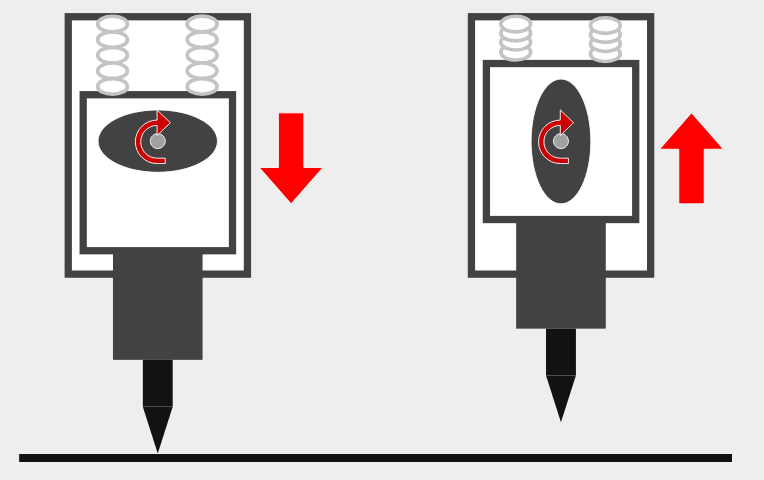
\includegraphics[width=0.66\linewidth]{Figures/pen-up-down-mechanism.png}
\caption{Cam-operated mechanism with the pen lowered and raised.}
\label{fig:des-penmechanism}
\end{figure}

The software checks the switch before energising the motor. If the desired state is already present, no pulse is required; an unnecessary rotation could move the pen away from the requested state. Otherwise the motor runs until the switch indicates the target or the timeout expires. The current control routine allows a 40\,ms overrun after confirmation of the raised state to seat the cam. This feedback operation differs from the G-code generator's settling dwell, which is described in Section~\ref{sec:des-gcode}.

The low-side BC337 circuit in Figure~\ref{fig:des-pencircuit} keeps the motor current out of the GPIO signal path. With a 1\,k$\Omega$ base resistor and the assumed $V_{BE}=0.7$\,V, Equation~\ref{eq:des-basecurrent} gives the approximate base current using the standard low-side resistor relation~\cite[section ``Why NPN Devices Are Used in Low-Side Switches]{rohmlowside2026}.
\begin{equation}
I_B=\frac{V_{\mathrm{GPIO}}-V_{BE}}{R_B}
=\frac{3.3-0.7}{1000}=2.6\ \mathrm{mA}.
\label{eq:des-basecurrent}
\end{equation}
The calculation in Equation~\ref{eq:des-basecurrent} establishes the nominal signal current only. It does not prove transistor saturation at motor startup or stall. The installed motor current, GPIO capability and transistor saturation conditions must be considered together~\cite{bc337ds}\designsourceflag{bc337ds}. Increasing base current without checking the GPIO rating would transfer the problem to the computer interface.
\begin{figure}[!htbp]\centering
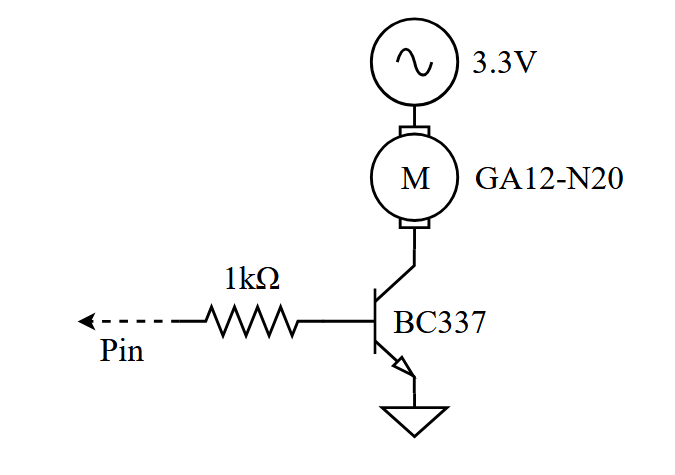
\includegraphics[width=0.60\linewidth]{Figures/pen-clicker-bc337-circuit.png}
\caption{Prototype pen-motor switching circuit supplied with the draft. Supply and protection details require confirmation against the installed circuit.}
\label{fig:des-pencircuit}
\end{figure}
The installed pen motor is powered from the ODROID's dedicated 3.3\,V supply pin, while the GPIO controls the transistor base through its resistor. The power pin and signal pin have different roles; moving the supply connection away from GPIO does not by itself establish that the rail can supply motor startup current. No flyback diode is fitted. Interrupting an inductive motor current can therefore impose a voltage transient on the switching stage~\cite[section ``Protection and Wiring Techniques]{rohmlowside2026}. A diode across the motor, reverse-biased during normal operation, would provide a recirculation path; its current and voltage ratings must be selected from the motor and supply conditions. This is a limitation of the installed circuit, not a protection feature already implemented.
\designgap{Measure pen-motor running/startup current and confirm the 3.3 V rail's available capacity. The user reports 10 kOhm pull-downs; confirm whether one is fitted at the transistor base as well as at switch inputs. Replace the prototype image with correct DC notation and actual installed components. Record the reason the motor-suppression diode was omitted before final submission.}

\subsubsection{End stops, homing and dimensional calibration}
\label{sec:des-calibration}
Four switches define the minimum and maximum travel of the two axes. Each is connected as an active-high input with a 10\,k$\Omega$ pull-down, as shown in Figure~\ref{fig:des-switch}. The pull-down defines the input while the contact is open. With the contact closed, its current is $3.3/10000=0.33$\,mA and dissipation is approximately 1.1\,mW. The resistor is between input and ground, so it does not limit fault current if the GPIO is incorrectly configured as an output driven low.
\begin{figure}[!htbp]\centering
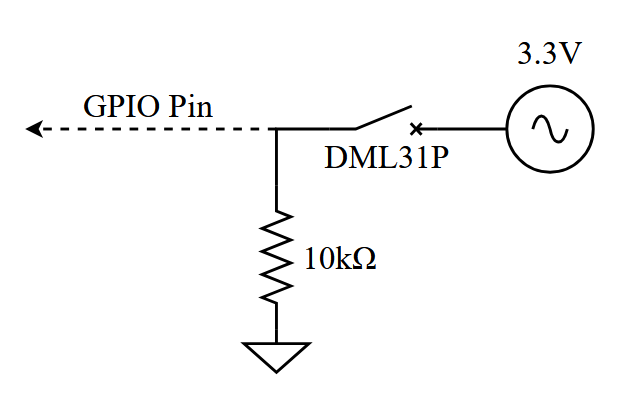
\includegraphics[width=0.62\linewidth]{Figures/endstop-switch-pulldown-circuit.png}
\caption{Active-high switch input with a 10\,k$\Omega$ pull-down.}
\label{fig:des-switch}
\end{figure}

The control routine confirms a high reading with two further samples separated by 6\,ms. Requiring three consistent readings rejects brief transients, at the cost of waiting approximately 12\,ms when a potential trip is checked. Axis pulses are not continuously generated during this blocking check, so multiplying the full confirmation interval by the commanded feed would not correctly describe the software's movement during debounce. Physical stopping distance also depends on the mechanics; it requires a measurement rather than a software-delay calculation alone.

After startup, the step counters do not establish a known physical origin. Calibration therefore drives one axis towards either switch, reverses towards the other, and counts the switch-to-switch steps. Equation~\ref{eq:des-calibration} converts this count to the scale used for motion.
\begin{equation}
\kappa_x=\frac{N_x}{L_x},\qquad \kappa_y=\frac{N_y}{L_y},\qquad
n_x=\operatorname{round}[(x+e)\kappa_x].
\label{eq:des-calibration}
\end{equation}
Here $N_x,N_y$ are measured step counts, $L_x,L_y$ are the independently measured switch-to-switch travels, and $e=5$\,mm is the edge clearance. The corresponding expression applies to $y$. An axis retracts from the switch after calibration, and the origin lies inside the physical boundary. Absolute target counts are rounded and differenced against the tracked count, so rounding of one segment is not repeatedly accumulated as a new relative position error.

The recorded travel constants in the current code are $L_x=200.6$\,mm and $L_y=261.3$\,mm. With 5\,mm clearance on both ends, the software travel limits are 190.6 by 251.3\,mm before the writing margins are applied. These are configuration values describing the available travel; a separate calibration record is needed to state the measured microsteps per millimetre. The result of calibration is not retained as a valid position across a restart.

Calibration compensates for scale error, but it cannot correct an imprecise reference measurement. If the travel measurement has error $\delta L$, its first-order contribution to position error at commanded distance $x$ is given by Equation~\ref{eq:des-scaleerror}.
\begin{equation}
|\delta x|\simeq |x|\frac{|\delta L|}{L}.
\label{eq:des-scaleerror}
\end{equation}
For example, allocating 0.25\,mm to scale error over 190.6\,mm of $x$ travel requires the 200.6\,mm reference travel to be known to approximately 0.263\,mm. This allocation in Equation~\ref{eq:des-scaleerror} is a design budget, not a measured uncertainty. Switch repeatability, backlash, pen compliance and squareness require the remaining error allowance.

\subsubsection{Electrical integration and power distribution}
\label{sec:des-power}
The motor-driver supply is operated at 24\,V. The recorded supply-current indication is 0.35\,A, with the supply current limit set to 2.11\,A. These quantities have different meanings: the first is a reading at an operating condition, the second limits the available supply current, and neither specifies the winding-current regulation of an A4988. The observed 24\,V and 0.35\,A correspond to 8.4\,W at that supply output; this is not a peak-power rating or the total robot consumption unless all loads and the measurement condition are included.

The A4988 current-trip setting follows Equation~\ref{eq:des-current}~\cite[p.~9]{a4988ds}.
\begin{equation}
I_{\mathrm{trip,max}}=\frac{V_{\mathrm{ref}}}{8R_S}.
\label{eq:des-current}
\end{equation}
Here $R_S$ is the carrier's sense resistance and $V_{\mathrm{ref}}$ is the measured reference voltage. For illustration only, $R_S=0.10\,\Omega$ and a 1.00\,A trip setting would require $V_{\mathrm{ref}}=0.80$\,V. The actual setting depends on the installed resistor and reference voltage. Available torque and driver heating depend on that setting; the motor's 1.68\,A phase rating does not mean the driver is operating at 1.68\,A.

The reported resistor marking is tentatively R10, corresponding to 0.10\,$\Omega$ if confirmed. This supports the illustrative resistance in Equation~\ref{eq:des-current}, but does not supply the missing measured reference voltage. The ODROID uses its supplied mains adapter; its DC output rating is recorded separately from the 24\,V stepper supply. The dedicated ODROID 3.3\,V rail supplies the installed 3.3\,V loads, including the pen motor. The GPIO connections carry the associated control and feedback signals.

The complete wiring needs a defined common logic reference between the ODROID, drivers and pen circuit. Motor-current returns should not be confused with signal paths, and driver supply decoupling must be located at the driver rather than relying on long supply leads. Figure~\ref{fig:des-complete-circuit} provides the place for the final circuit with those connections and component values visible.
\begin{figure}[!htbp]\centering
\designasset{design-complete-circuit.pdf}{0.98}{Complete circuit with GPIO offsets/physical pins, 24 V motor rail, ODROID supply, pen supply, driver logic rails, switch resistors and protection components.}
\caption{Complete electrical circuit and power distribution.}
\label{fig:des-complete-circuit}
\end{figure}
\designgap{Confirm each driver's sense-resistor marking, measured Vref and cooling arrangement; record the ODROID adapter's DC output rating, the operating state during the 0.35 A reading, and fitted decoupling.}

\subsubsection{Image capture arrangement}
\label{sec:des-camera}
The image-processing input depends on the camera arrangement as well as the algorithms. A camera looking approximately normal to a flat page reduces perspective distortion, and a restrained page reduces local curvature that a single deskew angle cannot remove. The capture area must include the full writing region while keeping the relevant strokes large enough to survive the line crop and network resize. The proposal specifies well-lit operation; software illumination normalisation is intended to accommodate residual variation within that arrangement.

The USB capture path returns a saved image to the same classification routine used for uploads. This gives both inputs a common orientation and segmentation procedure. The installed camera position, page restraint and illumination arrangement are identified in Figure~\ref{fig:des-capture}.

The camera is specified as an 8\,MP USB autofocus unit with an IMX179 CMOS sensor and a $78^\circ$ field of view. Its supplied resolution specification is 3264 by 2488 pixels. The capture module opens the UVC device through OpenCV, reuses an active preview handle when available, and otherwise discards an initial sequence of five frames before saving the last readable frame. This gives the camera time to settle, but does not verify sharpness or autofocus convergence. The current routine does not explicitly request that advertised resolution, so the saved frame dimensions must be checked rather than equating sensor specification with operating resolution.
\begin{figure}[!htbp]\centering
\designasset{design-camera-arrangement.jpg}{0.70}{Photograph of the actual camera and page mount, labelled with working distance, page area and illumination direction.}
\caption{Page capture arrangement used to supply images to the processing pipeline.}
\label{fig:des-capture}
\end{figure}
\designgap{Verify the supplied camera specification against its label and saved frame dimensions; add working distance and mounting dimensions. Describe only the lighting arrangement actually used; do not claim a measured lux range without a measurement.}

\subsubsection{Hardware verification and practical limitations}
The purpose of hardware verification is to establish that a coordinate command produces the intended type of movement before handwriting is introduced. Axis-aligned lines expose scale and direction errors; diagonal lines expose coordinated stepping and frame geometry; repeated pen changes expose clearance and pressure problems. The square-and-triangle comparison already included in the draft is useful for this purpose (Figure~\ref{fig:des-shapetest}). Its visual agreement supports correct interpretation of the commanded shape, but does not by itself establish the proposal's absolute accuracy or repeatability specification.
\begin{figure}[!htbp]\centering
\begin{minipage}{0.47\linewidth}\centering
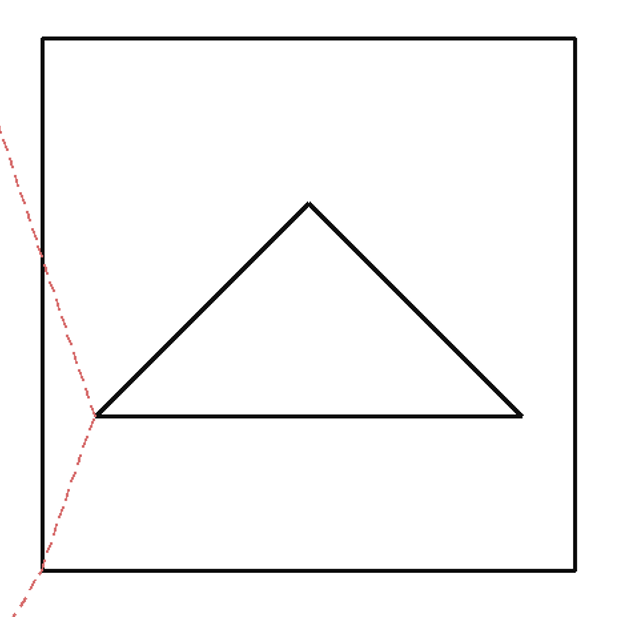
\includegraphics[width=\linewidth,height=0.23\textheight,keepaspectratio]{Figures/square-triangle-gcode-preview.png}\par(a) Commanded trajectory
\end{minipage}\hfill
\begin{minipage}{0.47\linewidth}\centering
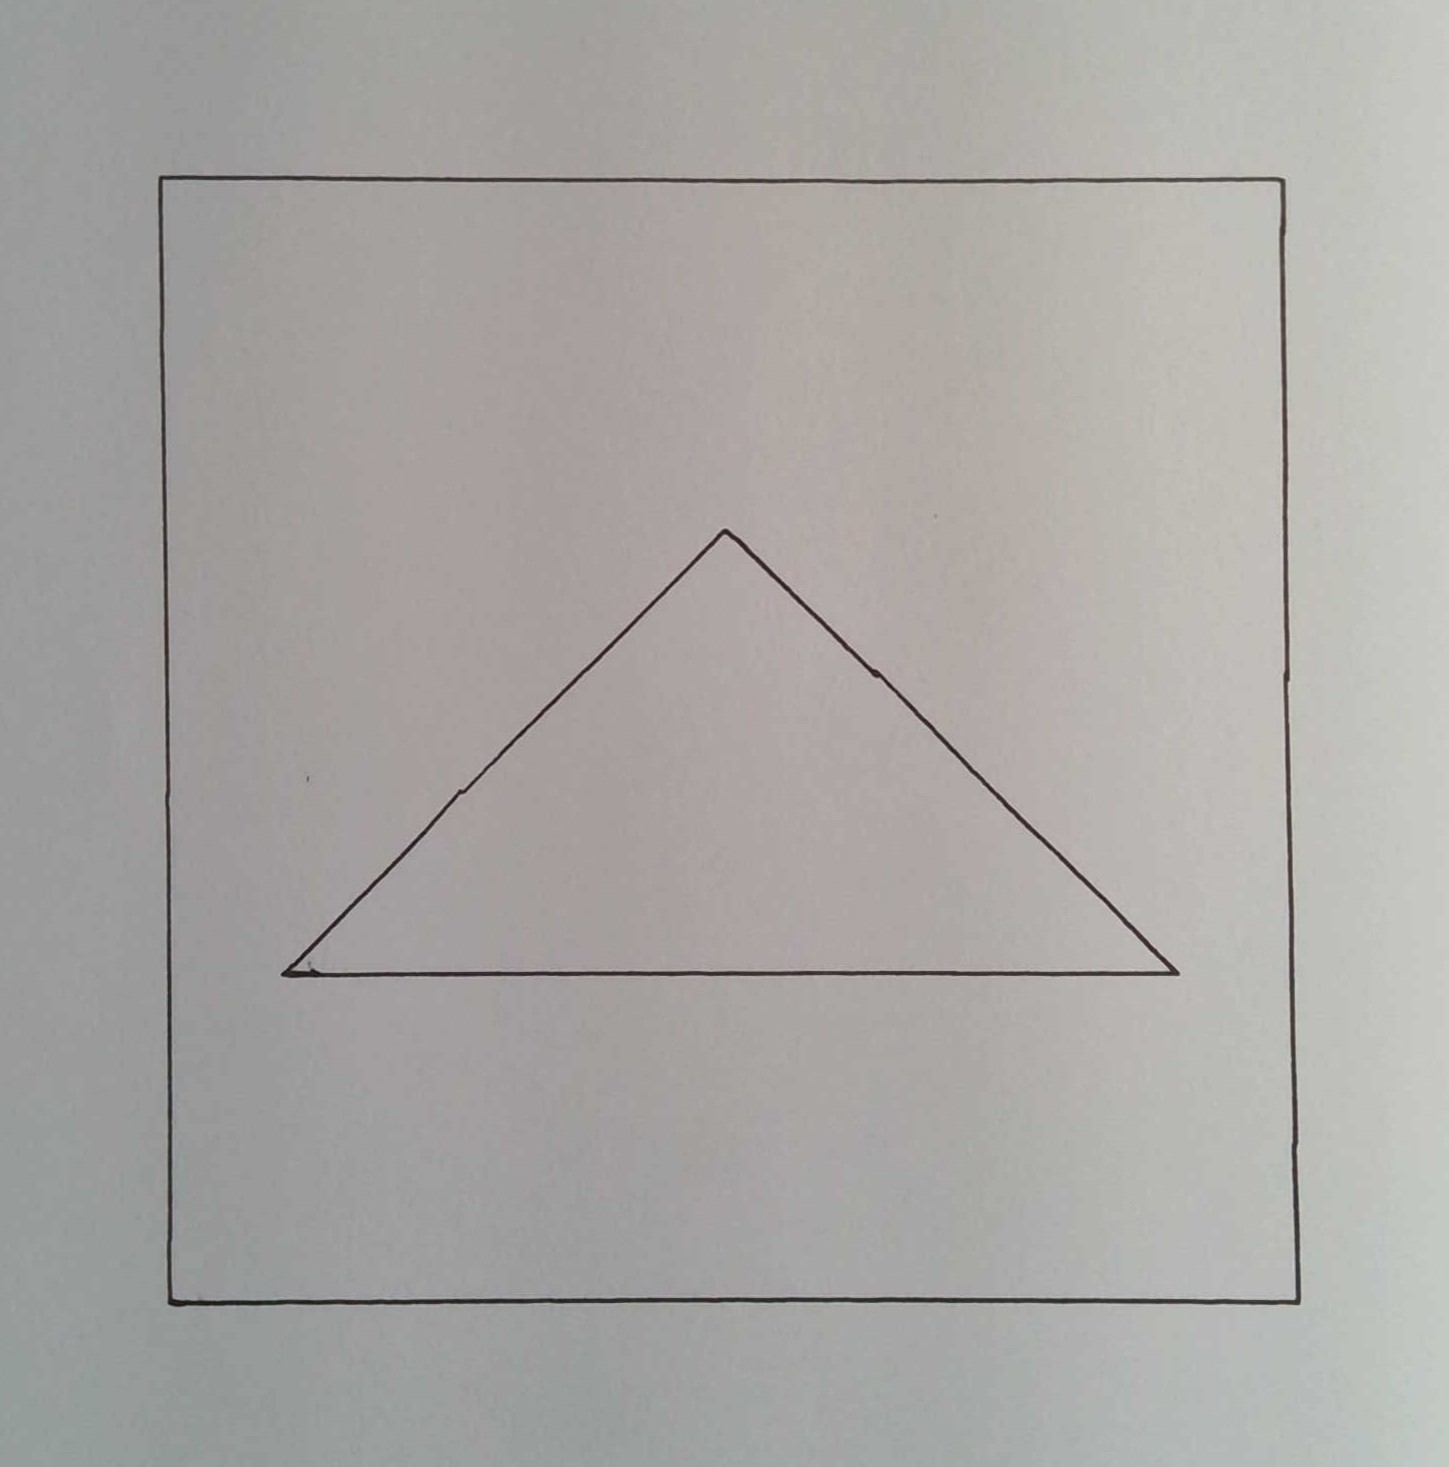
\includegraphics[width=\linewidth,height=0.23\textheight,keepaspectratio]{Figures/square-triangle-reproduced.jpg}\par(b) Physical drawing
\end{minipage}
\caption{Geometric commissioning example comparing the commanded path with the physical drawing. Formal positional qualification is reported in Results.}
\label{fig:des-shapetest}
\end{figure}

The design's principal strength is the direct relationship between orthogonal coordinates and motor displacement, combined with a mechanically shared drive on the two sides of the moving rail. Its principal uncertainties lie in physical compliance and open-loop execution. A missed step changes the actual position without changing the tracked count, and calibration cannot retrospectively recover where that happened. Controlled acceleration, a more consistent pulse scheduler and improved mechanical constraint are possible remedies, but their expected benefit must be separated from the performance of the implemented machine. The formal dimensional and repeated-drawing measurements belong in the Results section.
\FloatBarrier

\subsection{Page conditioning and line segmentation}
\label{sec:des-seg}
The recogniser requires an image containing one line of text. A photograph, however, may contain uneven illumination, a rotated page, printed rules, page edges and strokes extending between neighbouring lines. The purpose of this stage is to remove those disturbances while preserving the shape and relative spacing of the handwriting. The implemented sequence in \texttt{segment.py} works mainly on a half-resolution image, then returns to the full-resolution image to build the line crops.

\subsubsection{Input conditions and processing sequence}
The working image is a two-dimensional array of grey values. Where a colour array reaches the deskew routine, its channels are averaged to obtain brightness. Reducing the analysis image by averaging each $2\times2$ block reduces its pixel count by a factor of four. Averaging is preferred to selecting every second pixel because a thin stroke then contributes to the reduced image even if it falls between sampling positions. A further reduced mask is sufficient for the angle search, where only the arrangement of whole lines is needed.

The intermediate representations in Figure~\ref{fig:des-seg-stages} separate illumination correction, ink extraction, line boundaries and final crops. Inspecting these representations localises a missing stroke to the operation that removed it. The output includes the line images together with their order and diagnostic information such as skew angle, pitch and rejected crops.
\begin{figure}[!htbp]\centering
\designasset{design-segmentation-stages.pdf}{0.96}{One page shown as original image, normalised brightness, ink mask, cleaned mask with centres/seams, and resulting line crops. Use matching crops and a labelled scale.}
\caption{Processing stages used to obtain separate text-line images from a photographed page.}
\label{fig:des-seg-stages}
\end{figure}

A straight horizontal boundary is adequate only when there is a blank row between lines. Handwritten descenders and ascenders can overlap in vertical position without belonging to the same line. The chosen design therefore first locates the lines, then finds curved boundaries between them, and finally assigns complete ink pieces to a line. This is more appropriate than treating every connected ink component as a character, since cursive words may form a single component.

Algorithm~\ref{alg:des-segment} links the representations used in Figure~\ref{fig:des-seg-stages}. The order matters: rules and artefacts are removed before estimating final line centres, whereas faint-ink recovery occurs after ownership has been established.
\begin{designalgorithm}
\caption{Photographed page to ordered line crops}
\label{alg:des-segment}
\textbf{Input:} grey page on its chosen line axis. \textbf{Output:} crops, coordinates and diagnostics.
\begin{designsteps}
\item Estimate small skew on reduced ink coordinates; rotate the full and working grey images once.
\item Estimate local background, form the ratio mask and identify the paper region.
\item Remove printed runs and artefact pieces; retain the labelled component map.
\item Estimate line pitch and centres; find minimum-cost seams between adjacent centres.
\item Assign ink ownership and correct small detached or misplaced pieces (Algorithm~\ref{alg:des-ownership}).
\item Recover each crop from the full-resolution page, restricted by its ownership and local recovery neighbourhood.
\item Reject undersized crops and crops satisfying both solid-ink rejection tests.
\item Return ordered images, fixed-canvas inputs, bounding boxes and processing diagnostics.
\end{designsteps}
\end{designalgorithm}

\subsubsection{Lighting normalisation and ink extraction}
The first requirement is to distinguish ink from paper under an illumination gradient. A single threshold applied directly to brightness can classify a shadowed part of the page as ink while losing pale strokes elsewhere. Equation~\ref{eq:des-ratio} compares each pixel with its own local background estimate instead.
\begin{equation}
R(y,x)=\frac{G(y,x)}{\max[B_r(y,x),1]},\qquad
M(y,x)=\mathbf{1}[R(y,x)<t^*].
\label{eq:des-ratio}
\end{equation}
Here $G$ is grey intensity on the 0--255 scale, $B_r$ is a square-window mean with radius $r$, $R$ is normalised brightness, and $M$ is the binary ink mask. The floor of 1 prevents division by zero in black regions. The code uses $r=\max(8,\min(40,\operatorname{round}(H/41)))$, where $H$ is the working-image height. The radius follows image size within bounded limits: it must average over strokes without following their darkness as if it were illumination.

The mean is evaluated through a summed-area table~\cite{crow1984}\designsourceflag{crow1984}. For an exclusive prefix sum $S$, the window sum is obtained from four accesses, as shown in Equation~\ref{eq:des-integral}.
\begin{equation}
\Sigma_{[y_0,y_1)\times[x_0,x_1)}=
S(y_1,x_1)-S(y_0,x_1)-S(y_1,x_0)+S(y_0,x_0).
\label{eq:des-integral}
\end{equation}
The window area divides this sum to give $B_r$. Equation~\ref{eq:des-integral} makes the cost per window independent of its radius after the prefix image has been constructed. Edge replication is used by this local-mean routine so that the boundary is not darkened by artificial zero padding.

Otsu's criterion selects $t^*$ from the ratio histogram rather than from the original grey histogram~\cite{otsu1979}\designsourceflag{otsu1979}. Equation~\ref{eq:des-otsu} gives the between-class variance being maximised.
\begin{equation}
t^*=\arg\max_t\ \omega_0(t)\omega_1(t)
\bigl[\mu_0(t)-\mu_1(t)\bigr]^2.
\label{eq:des-otsu}
\end{equation}
Here $\omega_0,\omega_1$ are the histogram masses below and above a candidate threshold and $\mu_0,\mu_1$ are their means. The normalisation in Equation~\ref{eq:des-ratio} first brings paper towards a common level, allowing the global criterion in Equation~\ref{eq:des-otsu} to operate on a more consistent image. The implementation uses 256 bins over the clipped ratio range 0--1.2.

Large solid regions are then removed because the dark surround or a binder interior can survive thresholding without representing handwriting. The page region is estimated from its bright connected area, and long nearly horizontal or vertical ink runs are masked as printed structure. Run thresholds are expressed relative to line pitch, rather than fixed photograph dimensions. The horizontal and vertical limits are respectively 1.25 and 1.4 pitches. These are geometric heuristics: a long handwritten underline can satisfy the same condition as a printed rule, so the algorithm is designed for text extraction rather than preserving every mark on a page.

\subsubsection{Page orientation and skew correction}
Orientation is treated at two scales. A quarter turn changes which axis contains the line gaps; a small skew changes how sharply ink is concentrated along rows. For the quarter-turn decision, the code compares the fraction of nearly empty rows in the current image and its $90^\circ$ rotation. A turn is accepted only when the rotated score exceeds the original by a factor of 1.35. This margin avoids rotating a page merely because two weak scores differ slightly. Sparse or unusually arranged text can still make the row-gap evidence ambiguous.

After choosing the line axis, the deskew routine tests angles from $-4^\circ$ to $+4^\circ$ at $0.5^\circ$ spacing. Equation~\ref{eq:des-skew} gives its objective, related to projection-profile methods~\cite{postl1986}\designsourceflag{postl1986}.
\begin{equation}
\theta^*=\arg\max_\theta\sum_y p_\theta(y)^2,\qquad
p_\theta(y)=\sum_x M_\theta(y,x).
\label{eq:des-skew}
\end{equation}
Here $p_\theta$ is the row ink count at a candidate angle. Squaring favours concentrated rows over the same amount of ink spread across many rows. Rather than rotating the complete mask for every trial, the implementation maps ink coordinates to candidate rows and counts them. The selected rotation is then applied to the full and working grey images, and the mask is recomputed. This avoids repeatedly interpolating a binary image.

A page and its upside-down version have the same line-axis structure. The server therefore uses the reader to compare up to three sampled line crops in both directions. It compares the mean best-frame log score, reuses the selected readings and reverses line order when necessary. This is an orientation heuristic, not an independent measure of text correctness. A reader that is confidently wrong can select the wrong orientation, particularly when little text is available.

\subsubsection{Line detection and separation}
The line pitch $P$ provides the main scale reference for later decisions. A smoothed row profile is formed from the central writing region; candidate peaks must exceed 6\% of its maximum. The preferred estimate is the median distance between peaks, subject to a lower bound based on component height. This check prevents the ascender, body and descender bands of a single large line from being treated as separate line spacings. Autocorrelation and a component-height estimate provide fallbacks when direct gaps are unsuitable.

Line centres are selected in order of peak strength, with a minimum separation of $0.6P$. This suppresses several peaks within the same line. The code also supports merging peaks separated by a shallow valley, but that additional rule is not automatically active for every photographed page; its default threshold disables merging. The distinction matters because a rule that improves rendered text need not improve the shadows and artefacts of a real photograph.

Between each pair of centres, a minimum-cost seam crosses the image from left to right. The dynamic programme in Equation~\ref{eq:des-seam} follows the seam-carving principle~\cite[PDF p.~3, Sec.~3]{avidan2007}.
\begin{equation}
D(y,x)=C(y,x)+\min_{|d|\leq s}
\{D(y+d,x-1)+0.02|d|\}.
\label{eq:des-seam}
\end{equation}
Here $D$ is accumulated cost, $C$ is the local cost and $s=7$ is the allowed row change per column. Backtracking from the minimum final cost returns the boundary. Equation~\ref{eq:des-seam} penalises unnecessary vertical movement while allowing a boundary to bend around a descender.

The cost in Equation~\ref{eq:des-seamcost} strongly discourages crossing ink and weakly attracts the boundary to the space between line centres.
\begin{equation}
C(y,x)=4\widetilde M(y,x)
+0.012\left(\frac{y-y_m}{h_g}\right)^2.
\label{eq:des-seamcost}
\end{equation}
Here $\widetilde M$ is the mask after a closing operation, $y_m$ is the midpoint of the neighbouring centres and $h_g$ is half their separation. The closing radius is $\max(2,\lfloor0.07P\rfloor)$ pixels. Closing fills narrow gaps that would otherwise let a seam enter a stroke, without simply treating a thick dilation around every letter as real ink. In Equation~\ref{eq:des-seamcost}, the midpoint term resolves low-ink alternatives; it is deliberately much weaker than the ink penalty. The constants express the chosen preference, while the examples in Section~\ref{sec:des-segverify} must establish whether that preference produces useful boundaries.

\subsubsection{Ink ownership and classifier crop preparation}
Seams initially divide the image into bands, but a pixel-by-pixel cut can separate a dot from its stem or clip a curved descender. Connected-component ownership therefore refines the band assignment. Components are found with row runs and union operations, following connected-component labelling principles~\cite[pp.~476--479]{rosenfeld1966}. The implementation includes diagonal contact, giving eight-connected components. Large pieces can still contain writing from more than one line, so component labelling alone is not a complete line assignment.

Algorithm~\ref{alg:des-ownership} summarises the correction order. For a component spanning several bands, a band holding at least 15\% of its in-band ink is substantial. The uppermost substantial band supplies the reference owner for small-piece corrections; otherwise the largest overlap is used. Large components are not indiscriminately moved into that band: their pixels retain seam-band assignment except where the small-piece and narrow-tail rules apply. This distinction preserves a word's main body while recovering a protruding part.
\begin{designalgorithm}
\caption{Refining seam bands into ink ownership}
\label{alg:des-ownership}
\textbf{Input:} ink mask, components, seams, line centres and pitch $P$.
\begin{designsteps}
\item Count each component's pixels in each band; identify substantial overlaps and narrow minor tails.
\item Reject remote specks; move eligible small pieces towards nearby line bodies.
\item Associate compact dots with a plausible stem below, using pitch-scaled size and gap tests.
\item Form the initial ownership image, retaining band assignments for large pieces.
\item Inspect raw components to recover dots incorrectly grouped with writing above.
\item Recover enclosed ring-like marks with a plausible stem on the neighbouring line.
\item Reassign residual fragments lacking ink in their own line's body band, respecting protected earlier corrections.
\item Return one line index per owned ink pixel; unowned pixels remain excluded.
\end{designsteps}
\end{designalgorithm}

An \texttt{i} dot between two text lines illustrates the need for this sequence. A seam may put it with the upper line because of its vertical position, while a stem below supplies evidence for the lower line. Closing used for component analysis can also join the dot to an unrelated descender; the raw mask is therefore revisited rather than treating the closed component as unquestionable evidence. A ring-shaped mark needs the additional hole test so that an open hook is not treated as a detached loop. These are geometric decisions with ambiguous cases, rather than knowledge of the intended character.

The final crop is built from the full-resolution image and the refined ownership map. Contrast adjustment improves faint ink, while ownership restricts recovery so that strengthening one line does not simply pull a neighbouring stroke into it. The recogniser receives an aspect-preserving fit on a 64 by 640 canvas. Equation~\ref{eq:des-fit} defines the common scale for an original crop of height $h$ and width $w$.
\begin{equation}
a=\min\left(\frac{64}{h},\frac{640}{w}\right),\qquad
(h',w')\simeq(ah,aw).
\label{eq:des-fit}
\end{equation}
Remaining space is padded white, with the ink left-aligned and vertically centred. The shared scale in Equation~\ref{eq:des-fit} avoids stretching narrow letters differently from wide ones. Very long lines, however, become short in height when fitted to the width limit, which reduces the detail available to the networks.

The full-resolution crop uses a soft interpolation of its own ink mask to avoid jagged cut edges. A separate ownership exclusion is resized with nearest-neighbour interpolation: interpolating a yes/no ownership decision could partly return a neighbour's ink. Local thresholding can recover faint strokes within a neighbourhood of this line, but cannot recover ink already assigned to another line. Contrast is stretched between a robust ink level and paper level, followed by a darkness exponent of 0.55. This strengthens faint writing without replacing its geometry with a solid rectangular band.

The final solid-crop guard rejects a crop only when its dark-pixel fraction exceeds both 15\% and three times the page's median crop fraction. Requiring both prevents one unusually dense but genuine line from being rejected merely because other lines are sparse. It also prevents a shadow surviving as a confident writer vote in Section~\ref{sec:des-integration}.

\subsubsection{Segmentation verification and limitations}
\label{sec:des-segverify}
The verification comparison in Figure~\ref{fig:des-seg-variation} uses the same page under normal lighting, uneven lighting and a small rotation. Holding the writing fixed separates capture disturbances from differences between writers. The relevant observations are whether ink remains connected, whether the expected line count is recovered, and whether ascenders, descenders and dots stay with their own lines.
\designgap{Insert the matched capture examples and describe the actual observed differences. This comparison has not been performed as part of the present revision.}
\begin{figure}[!htbp]\centering
\designasset{design-segmentation-variation.pdf}{0.95}{Matched photographs of one page under normal/uneven lighting and small rotation, with selected line crops showing which disturbances are corrected and which remain.}
\caption{Effect of capture variation on conditioning and line separation for the same page.}
\label{fig:des-seg-variation}
\end{figure}

The scale-based thresholds and curved boundaries accommodate changes in handwriting size and overlapping vertical extents without assigning every page a fixed pixel spacing. Their assumptions also define the limitations. Highly irregular line spacing weakens a single pitch estimate, touching strokes from two lines can defeat component ownership, and sparse pages provide weak orientation evidence. Severe perspective or page curvature is not corrected by a global rotation. Improving the mount addresses the latter at source; more general page rectification would add processing and require its own verification.
\FloatBarrier

\subsection{Neural network design, training and classification}
\label{sec:des-class}
The classification stage has two outputs: the text in a line and the identity of its writer. Both depend on stroke features, but text recognition must preserve their horizontal order while writer identification must combine evidence across the line. Two networks therefore use the same convolutional architecture with different heads. The recogniser follows the CNN--BiLSTM approach of Kizilirmak and Yanikoglu~\cite[pp.~4--5]{kizilirmak2023}; the project implements and integrates that architecture with its own preprocessing, training and handwriting-reproduction pipeline.

\subsubsection{Training data, labels and evaluation separation}
Public IAM handwriting~\cite{marti2002}\designsourceflag{marti2002} and the photographed personal contributions provide examples with known text and writer identity. Public line images supply text-recognition training data, while writer-labelled pages and the personal samples support writer identification and style extraction. The eleven writers selected for the reported evaluation and intended demonstration are six database writers (150, 152, 153, 384, 552 and 588) and five personal contributors. A stored profile, a classifier output class and an evaluated writer are different objects; the checkpoint's recorded class mapping defines how its output indices are interpreted.

The data pipeline pairs every crop with its transcript and writer label. The same preparation functions are used by the first-principles and framework training routes so that a comparison does not silently change segmentation or label handling. Blank or unusable labelled lines are excluded. Characters outside the configured alphabet are filtered by the label encoder; they cannot be recognised as separate output symbols unless the alphabet and output layer are extended.

The page-based writer dataset holds out an IAM page per writer, while the personal data use a fixed-seed 15\% line split. A page split and a line split provide different separation: a held-out personal line can share camera conditions, page background and writing session with training lines. It is therefore appropriate to describe those samples as held-out lines, rather than as wholly unseen capture sessions. Augmented versions of a sample must remain within its assigned training partition.

Preparing labelled public forms also requires excluding printed prompts and signatures before pairing detected lines with the transcript. A plausible crop count is insufficient if printed text has displaced that pairing. The form-boundary preparation and the handwriting line segmenter therefore serve different purposes.

Glyph extraction introduces another possible overlap. A writer profile fitted from an evaluation page would already contain letterforms from that page, changing the meaning of a subsequent reproduction comparison. Evaluation separation therefore concerns both the classifier's training inputs and the profile's source pages, not only the split used by the network trainer.

A writer-model holdout does not automatically exclude those lines from the reader's separately sourced public corpus. Source-line identifiers must therefore be reconciled across both training manifests before a combined recognition result can be described as unseen-input performance. The line counts alone cannot establish that separation.
The eleven-writer classifier dataset contains 1186 labelled lines, including 517 IAM lines, partitioned into 1031 training and 155 held-out lines. The remaining 669 lines are photographed contributions. These counts describe writer-model preparation, not the much larger reader's public-line corpus. The final reader uses a joint corpus of Teklia pre-cut IAM lines and the five photographed writers. Its exact training and validation counts remain to be recovered.
\designgap{Record reader split counts and the source pages used to construct final glyph profiles. Keep the reported writer holdout distinct from a wholly independent capture-session test.}

\subsubsection{Shared convolutional feature extractor}
The input tensor has dimensions $(B,1,64,640)$, where $B$ is batch size. The grey crop is inverted and scaled to $[-1,1]$, making dark ink positive and white padding negative. Table~\ref{tab:des-backbone} gives the implemented feature-map dimensions. Two pooling operations reduce the width to 160 positions; there is no third spatial pooling stage before height is collapsed.
\begin{table}[!htbp]\centering\small
\begin{tabularx}{\linewidth}{|l|X|l|}
\hline\textbf{Stage}&\textbf{Operation}&\textbf{Output excluding batch}\\\hline
Input&Aspect-preserving line fit and intensity scaling&$1\times64\times640$\\\hline
1&Two $3\times3$ convolutions, each with batch normalisation and ReLU; $2\times2$ max pool&$32\times32\times320$\\\hline
2&Four convolution/normalisation/ReLU blocks; $2\times2$ max pool&$64\times16\times160$\\\hline
3&Six convolution/normalisation/ReLU blocks&$128\times16\times160$\\\hline
Height reduction&Maximum over the remaining height&$128\times1\times160$\\\hline
\end{tabularx}
\caption{Implemented convolutional backbone shared in architecture by the text and writer networks. The two models have separately trained parameters.}
\label{tab:des-backbone}
\end{table}

The layer operation in Equation~\ref{eq:des-conv} shows what the numerical implementation evaluates. For output channel $o$, the input-channel and kernel sums combine into one feature value.
\begin{equation}
z_{o,y,x}=b_o+\sum_c\sum_{i,j}W_{o,c,i,j}X_{c,y+i,x+j}.
\label{eq:des-conv}
\end{equation}
Here $W$ is the learned kernel, $b$ its bias and $X$ the padded input. Equation~\ref{eq:des-conv} is the cross-correlation convention used by the implementation. Image patches are rearranged into a matrix and multiplied by flattened kernels, rather than evaluating a Python loop for every multiply. This follows the matrix formulation of convolution~\cite{chellapilla2006}\designsourceflag{chellapilla2006}. The choice improves the practicality of the numerical route while leaving the layer's calculation visible.

Batch normalisation evaluates Equation~\ref{eq:des-bn}, with channel statistics computed over the batch and spatial dimensions during training~\cite[PDF pp.~4--5, Alg.~1]{ioffe2015}.
\begin{equation}
\widehat z=\frac{z-\mu_B}{\sqrt{\sigma_B^2+\epsilon}},\qquad
y=\gamma\widehat z+\beta.
\label{eq:des-bn}
\end{equation}
Here $\gamma,\beta$ are learned channel parameters and $\epsilon$ stabilises division. At inference, stored running statistics replace $\mu_B,\sigma_B^2$, making Equation~\ref{eq:des-bn} a fixed affine operation. The following ReLU applies $\max(0,y)$ and max pooling retains the largest feature in each local window. These operations progressively convert pixel neighbourhoods into learned responses while reducing the spatial size passed to the task heads.

\begin{figure}[!htbp]\centering
\designasset{design-network-architecture.pdf}{0.96}{One architecture diagram with the 64x640 input and shared layer pattern branching into the BiLSTM/CTC reader and width-pooling/writer head. Include tensor dimensions.}
\caption{Architecture of the text reader and writer classifier.}
\label{fig:des-network}
\end{figure}
Figure~\ref{fig:des-network} makes the different uses of horizontal position explicit. The term ``shared'' refers to architecture and numerical building blocks; it does not mean that the trained writer classifier uses the reader's current weight tensors.

\subsubsection{Text recognition using sequence modelling and CTC}
The text head treats the 160 feature columns as a sequence. Each column contains 128 features after height pooling. Two bidirectional LSTM layers, each with 256 hidden units per direction, combine evidence from both sides of a character before a linear head produces scores over the alphabet and the blank class. The configured alphabet contains 73 characters, giving 74 output classes including blank. The chosen input geometry and decoding are part of this project's implementation rather than an assertion that every setting in the reference study was reproduced.

The LSTM state update in Equation~\ref{eq:des-lstm} retains an additive memory path~\cite[p.~5, Eqs.~(9)--(11)]{graves2013}.
\begin{equation}
c_t=f_t\odot c_{t-1}+i_t\odot g_t,\qquad
h_t=o_t\odot\tanh(c_t).
\label{eq:des-lstm}
\end{equation}
Here $c_t$ is cell state, $h_t$ is hidden output, $i_t,f_t,o_t$ are sigmoid input, forget and output gates, and $g_t$ is the candidate update. Each is computed from the current feature vector and previous hidden state. The implementation omits the additional cell-to-gate peephole connections shown in the cited source. The backward direction applies the same type of recurrence to the reversed sequence, and the two outputs are concatenated. Equation~\ref{eq:des-lstm} explains why the implemented reader has sequence state in addition to convolutional features.

The gates are obtained from one matrix calculation, split in input, forget, candidate and output order: $[a_i,a_f,a_g,a_o]^T=W_xx_t+W_hh_{t-1}+b_x+b_h$. Sigmoid is applied to $a_i,a_f,a_o$ and $\tanh$ to $a_g$. Concatenating both directions gives 512 features per frame; the second recurrent layer therefore receives 512 inputs rather than the first layer's 128. At inference the entire line is available, so using right-hand context does not require predicting future input.

CTC trains from a line transcript without requiring character positions~\cite[PDF pp.~2--3]{graves2006}. Equation~\ref{eq:des-ctc} sums the probabilities of frame paths that collapse to the target string.
\begin{equation}
\mathcal L_{\mathrm{CTC}}=-\log\sum_{\pi:\mathcal B(\pi)=\boldsymbol\ell}
\prod_{t=1}^{T}p_t(\pi_t).
\label{eq:des-ctc}
\end{equation}
Here $p_t(k)$ is the frame probability for symbol $k$, $\boldsymbol\ell$ is the transcript, and $\mathcal B$ merges consecutive repeats before deleting blanks. For example, the path $a,a,\varnothing,b,b$ collapses to ``ab'', while $a,\varnothing,a$ preserves ``aa''. The dynamic programme uses blank-interleaved states with transitions that stay, advance one state, or skip a blank when the adjacent labels differ. Arithmetic is performed in log space to avoid multiplying many small probabilities.

The implementation produces $T=160$ frames. A target with $L$ labels and $r$ adjacent repeated-label pairs requires at least $L+r$ frames. The extended lattice has $2L+1$ states, but not every state must be visited; that number is not a universal minimum sequence length. At inference, greedy frame decisions are collapsed by the same rule. This avoids a dictionary or language model, but a locally plausible wrong frame path can remain wrong even where a beam search could recover an alternative.

Algorithm~\ref{alg:des-ctc} describes the numerical loss and derivative. Let $\alpha_{t,s}$ include the current state's emission, while $\beta_{t,s}$ accounts only for emissions after frame $t$. The derivative used by the implementation is then Equation~\ref{eq:des-ctcgrad}, with the occupancy convention obtained by adapting the CTC forward--backward derivation~\cite[PDF pp.~5--6]{graves2006}.
\begin{equation}
q_{t,k}=\sum_{s:\ell'_s=k}\exp(\alpha_{t,s}+\beta_{t,s}-\log Z),
\qquad \frac{\partial\mathcal L}{\partial z_{t,k}}=p_t(k)-q_{t,k}.
\label{eq:des-ctcgrad}
\end{equation}
Here $Z$ is the total probability of admissible target paths, $z$ denotes logits and $q$ is posterior class occupancy. The convention for $\beta$ avoids counting the current emission twice. Equation~\ref{eq:des-ctcgrad} is averaged over the batch in the trainer, without an additional target-length division.
\begin{designalgorithm}
\caption{Numerical CTC loss and logit gradient}
\label{alg:des-ctc}
\textbf{Input:} frame logits and encoded transcript for each batch item.
\begin{designsteps}
\item Compute log-softmax by subtracting each frame's largest logit before exponentiation.
\item Interleave the target labels with blanks; initialise unreachable lattice states to $-\infty$.
\item Initialise the first blank and first label at frame zero.
\item Advance forward scores using log-sum-exp over stay, advance and permitted skip transitions.
\item Obtain $\log Z$ by combining the two admissible final states.
\item Initialise final backward scores to zero; recurse backwards, including the next frame's emission.
\item Sum posterior occupancies for all states emitting each class, as in Equation~\ref{eq:des-ctcgrad}.
\item Return mean negative $\log Z$ and batch-averaged logit gradients.
\end{designsteps}
\end{designalgorithm}

For the illustrative transcript ``letter'', the two adjacent \texttt{t}s require separate emission runs with a blank between them. Advancing directly from one \texttt{t} state to the next would collapse to a single character, so that skip transition is forbidden. This same restriction is retained during forced alignment in Section~\ref{sec:des-alignment}; training sums admissible paths, whereas extraction selects one.

\subsubsection{Writer identification and stroke normalisation}
\label{sec:des-shapenamer}
Writer identification should combine the shape evidence distributed along a line. It therefore averages the 160 column features rather than passing them through a sequence decoder. A 128-element feature vector is mapped through a 96-unit hidden layer, ReLU and a final $K$-class output. Dropout with probability 0.2 is active in the hidden head during training and omitted during inference~\cite[pp.~1931, 1934]{srivastava2014}. Here $K$ is the number of writers represented by that checkpoint.

The initial classifier operated on handwriting as photographed and performed well on those samples. However, such images contain more than letter shape: pen width, darkness and the capture process can also distinguish writers. The gantry uses its own pen, so reproducing the selected writer's geometry does not reproduce the same ink appearance. A classifier that relies on those cues would therefore provide an unsuitable basis for judging whether the robot preserved the writer's style.

The later classifier uses stroke-normalised input. Ink is binarised, reduced to a centreline with Zhang--Suen thinning~\cite[p.~237]{zhang1984}, then expanded to a controlled width before the fixed-canvas fit. Equation~\ref{eq:des-strokenorm} describes the implemented transformation.
\begin{equation}
I_s=255\left[1-\delta_k\bigl(\operatorname{thin}(M)\bigr)\right],\quad
w=\operatorname{clip}\bigl(\operatorname{round}(\rho h_x),2,9\bigr),\quad
k=2\lfloor w/2\rfloor+1.
\label{eq:des-strokenorm}
\end{equation}
Here $h_x$ is estimated x-height, $\rho$ is the selected width fraction and $\delta_k$ is square dilation with an odd $k$-pixel kernel. The actual discrete kernel is important: nearby fractions can produce exactly the same transformed image. The code contains a default fraction of 0.14 and supports explicit training widths; the final model and its preprocessing must use matching settings.

The stroke-normalised classifier is used for writer identification and synthesis evaluation in the final design described here. This reduces dependence on ink appearance while retaining the letter geometry that the gantry can reproduce. It does not make the classifier completely independent of capture conditions, since thresholding and skeletonisation can themselves change a faint or touching stroke. It also removes potentially useful evidence from original handwriting, making the choice a deliberate trade-off between photograph-specific discrimination and consistency across original and reproduced writing.

Figure~\ref{fig:des-strokenorm} shows this transformation on existing real crops. The comparison makes the individual operations visible: binary extraction defines what ink is retained, thinning reduces it to a centreline, and dilation restores a controlled width. A matched ink-versus-shape comparison on original and reproduced samples can then test the reason for the choice without substituting classifier confidence for independent stylistic agreement.
\begin{figure}[!htbp]\centering
\designasset{design-stroke-normalisation.pdf}{0.98}{Two real writer crops shown as original ink, binary mask, skeleton and fixed-width redraw.}
\caption{Stroke-normalisation stages on selected Owen and Yeukita crops at the selected width fraction of 0.17.}
\label{fig:des-strokenorm}
\end{figure}
\designgap{Add a matched ink-versus-shape design comparison when available; do not compare different writer populations as if only preprocessing changed. Verify the selected checkpoint's preprocessing in the final submitted configuration.}

The width-selection tooling separates deterministic preparation from repeated learning. It skeletonises and redraws each crop once per candidate width, saving images together with writer names, labels and split membership. Training then augments those prepared images each epoch. Reusing the split and initialisation isolates width more effectively than changing width, population and sampling together. The preparation code records cases where normalisation returns no usable ink and the raw crop is retained; these fallbacks should be counted when interpreting a nominally shape-based dataset.

Table~\ref{tab:des-widthselection} records the supplied eleven-class validation sweep. All four runs had a 50-epoch budget and used the framework writer model on a Google Colab T4 GPU. The reported epoch is the best saved epoch, not the stopping epoch. The 0.17 setting gave the highest held-out accuracy in this sweep and defines the selected eleven-writer configuration; this is a preprocessing choice evaluated on validation data, not the integrated robot's writer-identification result.
\begin{table}[!htbp]\centering\small
\begin{tabular}{|c|c|c|}
\hline\textbf{Width fraction $\rho$}&\textbf{Best saved epoch}&\textbf{Held-out writer accuracy}\\\hline
0.06&38&98.06\%\\\hline
0.09&43&97.42\%\\\hline
0.11&39&98.06\%\\\hline
0.17&43&99.35\%\\\hline
\end{tabular}
\caption{Stroke-width selection using the same eleven-writer population and held-out partition.}
\label{tab:des-widthselection}
\end{table}
The selected checkpoint stores its width as 0.17. Both preparation and inference for that configuration must use this value; the module default of 0.14 is not its training setting. Figure~\ref{fig:des-strokenorm} illustrates the selected transformation on existing crops. Reusing the held-out partition to choose width makes it model-selection data; an independent test set remains necessary for an unbiased final performance claim.

\subsubsection{Training procedure and model selection}
\label{sec:des-training}
Both networks are trained through their complete convolutional backbones and task-specific heads. Convolution weights use variance-scaled initialisation; normalisation scales begin at one and offsets at zero. Training-time augmentation changes line geometry while preserving its label. The implemented transforms include shear, small rotations, perspective changes and elastic distortion. These operations are applied only to the training view, while validation retains a consistent preprocessing path.

The text trainer supports public lines, page-derived lines and a joint source that mixes public and personal examples. In the joint configuration, a personal-sample fraction controls their representation rather than letting a much larger public dataset determine the entire batch distribution. The default fraction is 0.20. This is a sampling choice, not a claim that personal and public samples are interchangeable. Its value and the training source must accompany any comparison between checkpoints.

Table~\ref{tab:des-training} summarises the numerical training recipe exposed by the current implementation. The number of epochs is a run setting and should be reported from the actual training record, rather than taking a command-line default as the completed run.
\begin{table}[!htbp]\centering\small
\begin{tabularx}{\linewidth}{|l|X|X|}
\hline\textbf{Setting}&\textbf{Reader}&\textbf{Writer classifier}\\\hline
Objective&CTC loss&Cross-entropy\\\hline
Optimiser&RMSprop&AdamW\\\hline
Initial learning rate&$10^{-3}$ default&$10^{-3}$ default\\\hline
Weight decay&$10^{-5}$&$10^{-4}$\\\hline
Learning-rate schedule&Plateau reduction, factor 0.5, patience 5, minimum $10^{-5}$&Cosine annealing over the configured run\\\hline
Gradient-norm clipping&Not applied by the current NumPy text loop&Maximum norm 5\\\hline
Best-checkpoint criterion&Lowest validation loss&Highest validation accuracy\\\hline
\end{tabularx}
\caption{Training settings implemented in the first-principles trainer. Final run settings require their own training records.}
\label{tab:des-training}
\end{table}

Cross-entropy penalises the writer model's predicted probability of the true class. For label $y$ and probabilities $p_k$, its per-sample loss is $-\log p_y$, with logit derivative $p_k-\mathbf{1}[k=y]$~\cite[p.~6, Eqs.~(13)--(14)]{graves2013}. The CTC backward pass similarly relates each predicted frame probability to its target-state occupancy, calculated by forward and backward recurrences through the alignment lattice~\cite[PDF pp.~4--6]{graves2006}. These gradients are propagated through the task head and the convolutional stages; they are not supplied to the numerical trainer by automatic differentiation.

Validation runs with dropout disabled and stored normalisation statistics. A low training loss alone does not select the model. Separate checkpoint and best-model files preserve progress while retaining the selected validation model. Reproducible batching, declared splits and saved writer mappings support later evaluation, but comparable recipes do not imply identical weights or learning curves across implementations.

Algorithm~\ref{alg:des-train} identifies the operations actually required for a first-principles training batch. Forward caches store quantities needed by the derivatives, rather than rerunning stochastic augmentation or dropout during the backward pass.
\begin{designalgorithm}
\caption{One numerical training batch and validation checkpoint decision}
\label{alg:des-train}
\textbf{Input:} labelled training batch, parameters, optimiser state and task.
\begin{designsteps}
\item Prepare task-specific inputs and labels. The writer view normalises strokes and fits the canvas before random training augmentation; keep validation deterministic.
\item Evaluate convolution, training normalisation, ReLU and pooling; retain backward caches.
\item Reader: evaluate both recurrent directions and CTC. Writer: average width features, evaluate the hidden head and cross-entropy.
\item Propagate the loss derivative through the task head, reversing time through each recurrent direction where present.
\item Propagate through height reduction, convolution blocks and spatial pooling.
\item For the writer, clip the total gradient norm to 5; apply the configured optimiser update.
\item At epoch end, evaluate the fixed validation view with inference normalisation and no dropout.
\item Update the schedule and save progress; replace the best checkpoint only when its task-specific validation criterion improves.
\end{designsteps}
\end{designalgorithm}

\subsubsection{First principles and framework implementations}
\label{sec:des-implementations}
The first-principles route in \texttt{train.py} evaluates the forward pass, backward pass, loss and optimiser updates using explicit NumPy operations. NumPy supplies array arithmetic and matrix operations; it does not supply a convolutional network, automatic differentiation or a CTC training function in this route. The learned parameters are stored as named arrays. The inference module reads these arrays and evaluates the forward operations without requiring a machine-learning framework.

The framework route in \texttt{trainlibrary.py} expresses the corresponding networks using PyTorch layers and automatic differentiation. It uses the project's data preparation and parameter naming, and exports weights in the same archive layout for numerical inference. It provides a reference implementation and an alternative training route; claims about training speed need a matched timing comparison because the framework may use a different processor or accelerator.

The final reader weights and the supplied writer-model weights were trained using PyTorch and exported to named arrays. The selected eleven-writer stroke-normalised model also follows the framework route. The first-principles trainer is an implemented and numerically checked contribution, while the operational forward path is numerical inference. These are separate claims: the report does not attribute production of the supplied final weights to the NumPy trainer.

Matching the architecture is not sufficient to establish a matched training experiment. The current numerical CTC function averages unnormalised sequence losses across the batch, whereas the framework trainer constructs CTC with its default mean reduction, which normalises each sequence by target length before averaging~\cite[CTCLoss, ``Parameters]{pytorchctc}. The latter also enables zeroing of impossible-alignment losses. A controlled training comparison must match these conventions if learning-curve equivalence is claimed: target-length weighting changes the relative influence of short and long lines. This does not prevent common weight export or matched fixed-parameter verification.

The reader checkpoint is \texttt{paper\_cnn\_bilstm\_ctc\_joint\_best.npz}; the selected eleven-writer checkpoint is \texttt{author\_shape\_11\_pw170\_weights.npz}. The reader's training computer, completed epoch count and original learning-rate/batch settings are not preserved in the supplied record. The implementation defaults in Table~\ref{tab:des-training} must therefore not be presented as recovered settings for that historical run. Older classifier archives do not establish the selected eleven-class configuration merely because their filenames also contain ``shape''.

The two routes are summarised in Table~\ref{tab:des-implementations}. Both export named arrays for numerical inference, so the deployed forward calculation is independent of the training engine. Training provenance remains a separate property of each checkpoint: executing weights with the numerical reader does not establish which implementation produced them.
\begin{table}[!htbp]\centering\small
\begin{tabularx}{\linewidth}{|p{0.23\linewidth}|X|X|}
\hline\textbf{Aspect}&\textbf{First principles route}&\textbf{Framework route}\\\hline
Layer calculations&Explicit forward and backward operations&Framework modules and automatic differentiation\\\hline
Architecture&Project's reader and writer definitions&Corresponding layer pattern and parameter names\\\hline
Data preparation&Project crop, label and split functions&Uses the same preparation functions\\\hline
Weights for inference&Named array archive&Export to the same named array layout\\\hline
Verification role&Implementation being checked&Reference for matched numerical comparisons\\\hline
\end{tabularx}
\caption{Roles of the numerical and framework implementations.}
\label{tab:des-implementations}
\end{table}

Equation~\ref{eq:des-conv} and the shape progression in Table~\ref{tab:des-backbone} define the implemented forward calculation. Its numerical correspondence and the backward operations are checked separately in Section~\ref{sec:des-netverify}. This separation distinguishes a correct description of an architecture from evidence that its calculations were implemented correctly.

For one image, let $X_c$ contain flattened input patches, so the convolution becomes $Y=WX_c+b$. With output derivative $G$, Equation~\ref{eq:des-convback} supplies the two matrix derivatives used by the numerical route.
\begin{equation}
\frac{\partial\mathcal L}{\partial W}=GX_c^T,\qquad
\frac{\partial\mathcal L}{\partial X_c}=W^TG.
\label{eq:des-convback}
\end{equation}
Weight and bias derivatives are summed over the batch and output positions. Overlapping patch derivatives in Equation~\ref{eq:des-convback} are added back into the padded input, not overwritten. Max-pool derivatives return to the recorded maxima, width-average derivatives are distributed uniformly, and the LSTM backward pass accumulates both hidden-state and cell-state contributions through time. Appendix~\ref{app:des-implementation} records the remaining derivative conventions and optimiser calculations without repeating the architecture here.

The matrix formulation also has a memory cost. The first convolution's patch matrix contains $B(1)(3)(3)(64)(640)$ values. At batch size eight, its float32 storage alone is approximately 11.25\,MiB, before later-layer patches, activations or gradients. This calculated example explains why numerical array operations do not automatically imply a small training footprint. Training memory and the embedded forward-only inference footprint must be assessed separately.

\subsubsection{Network verification and design limitations}
\label{sec:des-netverify}
Verification separates numerical correspondence from learning performance. For the first, the implementations receive the same parameters and inputs, with matched precision, normalisation state and stochastic masks. Differences in logits, loss and gradients then test the implementation. A second experiment trains each route on the same split with recorded initialisation and settings, and compares learning behaviour and held-out predictions. These experiments answer different questions: separately trained weights can differ even when the underlying operations agree.

The existing comparison archive contains a controlled text experiment using 500 training lines, 40 validation lines and 40 test lines over 15 epochs. It is useful supporting evidence for the implementation, but it is not the final eleven-writer system evaluation. A separate archived double-precision comparison uses two random 64 by 640 inputs and identical initial weights, checking the reader and a thirteen-output writer head. Table~\ref{tab:des-numericalcheck} summarises its recorded values. The writer dropout is disabled for this comparison so that unrelated random masks do not dominate the difference.
\begin{table}[H]\centering\small
\begin{tabularx}{\linewidth}{|X|r|r|}
\hline\textbf{Recorded comparison metric}&\textbf{Reader}&\textbf{Writer head}\\\hline
Maximum logit difference / maximum magnitude&$2.12\times10^{-14}$&$3.04\times10^{-15}$\\\hline
Absolute loss difference&$1.14\times10^{-13}$&$1.78\times10^{-15}$\\\hline
Worst ranked gradient relative $L_2$ difference&$2.80\times10^{-13}$&$6.01\times10^{-14}$\\\hline
\end{tabularx}
\caption{Archived float64 implementation comparison from the CleanPipeline2 verification script. This is a controlled numerical check, not a final-model recognition result.}
\label{tab:des-numericalcheck}
\end{table}
The logit metric in Table~\ref{tab:des-numericalcheck} divides the largest absolute difference by the larger maximum magnitude, with a $10^{-8}$ denominator floor. Gradient differences are $\|g_N-g_T\|_2/\|g_T\|_2$, where $g_N$ and $g_T$ are numerical-route and framework gradients. Tensors whose maximum gradient magnitude is below $10^{-6}$ are retained in the archive but excluded from the worst-ranked summary: dividing roundoff by a nearly zero gradient gives an unhelpful relative error. These results support close agreement for that tested configuration; they do not establish equivalence for every input, code revision or training trajectory.
\designgap{Confirm applicability of the archived comparison to the submitted implementation and add the matched final training comparison. Obtain any missing final reader/writer comparisons from the existing project work.}

An additional check can compare an implemented derivative with the central difference in Equation~\ref{eq:des-gradcheck}.
\begin{equation}
g_i^{\mathrm{num}}=\frac{\mathcal L(\theta+\varepsilon e_i)
-\mathcal L(\theta-\varepsilon e_i)}{2\varepsilon}.
\label{eq:des-gradcheck}
\end{equation}
Here $\theta$ is a parameter vector, $e_i$ selects one component and $\varepsilon$ is a small perturbation. Equation~\ref{eq:des-gradcheck} requires care at ReLU or max-pool boundaries and with stochastic dropout. The input or mask must be controlled so that the two loss evaluations test the same local operation.

The main design limitations concern what the input and training population can support. Fixed-width fitting limits detail in long lines; a closed writer head always selects among its trained classes; and line-level personal holdout does not establish independence from page or capture conditions. Stroke normalisation improves consistency with the pen plotter but can destroy detail when thresholding or thinning fails. These limitations should be assessed through appropriate examples and held-out measurements, rather than by treating a high softmax probability as proof of generalisation. Formal recognition and writer-identification qualification remains in Results.
\FloatBarrier

\subsection{Style extraction and handwriting reproduction}
\label{sec:des-reproduction}
Recognising a line does not provide the motion needed to write it. The reproduction stage must recover usable pen paths from a writer's examples, store the properties that distinguish that writer, and assemble the paths into text that was not necessarily present in the examples. The chosen representation is a library of normalised glyph trajectories accompanied by line-level style measurements. It provides explicit control over scale and movement, while making the limits of character-based reproduction visible.

\subsubsection{Character alignment and glyph extraction}
\label{sec:des-alignment}
The extraction input is a line image and its known transcript. Character boundaries are not supplied as labels. Instead, the trained reader gives a probability distribution for every output frame, and forced alignment finds the highest-scoring CTC path consistent with the supplied text. This is a localisation problem: the transcript constrains which labels must occur, while the frame scores indicate where they most plausibly occur.

The alignment uses the same permitted transitions as the CTC training lattice, but maximises a path score instead of summing all path probabilities. Equation~\ref{eq:des-viterbi} gives the recurrence by replacing path summation in the CTC lattice with maximisation~\cite[PDF pp.~4--5]{graves2006}.
\begin{equation}
V(t,s)=\log p_t(\ell'_s)+\max_{r\in\mathcal P(s)}V(t-1,r).
\label{eq:des-viterbi}
\end{equation}
Here $\ell'$ is the blank-interleaved transcript and $\mathcal P(s)$ is the permitted predecessor set: stay, advance one state, or skip an admissible blank. Backtracking yields the frames assigned to each character. Equation~\ref{eq:des-viterbi} makes clear why correct text does not guarantee correct boundaries: several spatial allocations can remain plausible under the same transcript.

An output frame is converted through the network canvas to the original crop using the inverse of its aspect-preserving scale. If a frame edge is $t$ out of $T$ and the crop was scaled by $a$, its initial horizontal location is approximately $(640t/T)/a$, clamped to the source width. This undoes the resize rather than assuming that every crop occupied the complete 640-pixel width.

The initial boundaries are refined by looking for thin, low ink near the expected cut. Equation~\ref{eq:des-cutcost} describes the principal column cost in \texttt{ExtractLineGlyphs}.
\begin{equation}
C_x=\frac{\overline p_x}{q_{0.60}(\{\overline p_j:\overline p_j>0\})}
+1.15\operatorname{clip}\left(\frac{b-y_{\mathrm{top}}(x)}{h_x},0,3\right).
\label{eq:des-cutcost}
\end{equation}
Here $\overline p_x$ is smoothed column ink count, the denominator is its 60th percentile over positive counts, $b$ is baseline position, and $y_{\mathrm{top}}(x)$ is the highest ink row in that column. A denominator floor prevents division by zero. A true blank column is assigned zero cost. The search radius is approximately half an x-height, with a smaller penalty for distance from the initial boundary. The two terms in Equation~\ref{eq:des-cutcost} favour a narrow connector near the baseline over cutting through the body of a letter.

One shared boundary array is enforced to remain increasing, with a minimum cell width of $\max(1,0.08h_x)$ pixels. Independently snapping neighbouring boundaries could place both at the same gap and create an empty glyph. Figure~\ref{fig:des-alignment} relates the initial alignment and refined cuts to the resulting character shapes.
\begin{figure}[!htbp]\centering
\designasset{design-glyph-alignment.pdf}{0.96}{Known transcript above two real line crops; initial CTC locations and refined cut columns distinguished; show resulting glyphs beneath, including a difficult cursive boundary.}
\caption{Transcript-constrained character localisation and refinement of glyph boundaries.}
\label{fig:des-alignment}
\end{figure}

\subsubsection{Skeleton tracing and pen path construction}
Ink is an area, whereas the gantry needs a path. Zhang--Suen thinning reduces the line mask to a one-pixel centreline~\cite[p.~237]{zhang1984}. The complete line is thinned before character cells are separated. Thinning each cut cell independently would introduce an artificial image edge at every character boundary and could change the recovered centreline there.

The skeleton is treated as a graph: adjacent ink pixels form edges, and endpoints and junctions determine where paths begin or split. Redundant diagonal edges are suppressed when an orthogonal route already connects the same local pixels. The default tracer first splits paths at junctions, prunes short dangling spurs, then greedily rejoins nearby ends with a continuation angle below $75^\circ$. Thus the default is not simply one pen lift per junction. A separate through-junction tracer exists but is not enabled by default. Neither procedure establishes natural pen order: the image records final ink, and several stroke sequences can create the same graph.

Traced paths are divided at the character boundaries and simplified while limiting geometric deviation, following the polyline-simplification principle of Douglas and Peucker~\cite{douglas1973}\designsourceflag{douglas1973}. Short spurs and cut ligature tails require care because a genuine small stroke can resemble a skeleton artefact. Isolated dots may thin to a single point with no traceable edge; these are recovered as short paths rather than silently discarded.

A detached \texttt{t} or \texttt{f} crossbar can extend over the next character cell. The extractor checks its width, flatness and height and, when the configured crossbar rule applies, assigns the complete bar to the corresponding letter instead of splitting it at a vertical cut. Such an overlap is not recorded as an in-word pen connection. Without this distinction, a crossbar would both contaminate the next glyph and inflate the profile's connectedness.

Each glyph is stored relative to its left boundary and the line baseline. Equation~\ref{eq:des-glyphcoords} defines the normalised coordinate frame.
\begin{equation}
v=\frac{b-y}{h_x},\qquad
u=\frac{x-x_L}{h_x}-v\tan\phi.
\label{eq:des-glyphcoords}
\end{equation}
Here $x_L$ is the cell's left edge, $h_x$ is x-height and $\phi$ is the estimated writing slant. In Equation~\ref{eq:des-glyphcoords}, image rows increasing downwards become glyph height increasing upwards. Removing slant at storage allows the writer's slant to be reapplied during placement without making every spacing measurement depend on shear. The glyph can then be drawn at a chosen physical x-height instead of a fixed number of source pixels.

Entry and exit positions are recorded along with whether the skeleton crosses a character boundary. This distinguishes a measured original connection from a merely small visual gap. The extracted paths still represent a geometric reconstruction, rather than the writer's true pen trajectory: retracing, pressure and movement direction cannot generally be recovered uniquely from a static image.

\subsubsection{Glyph selection and library quality}
The library must retain variation without giving every cut equal credibility. A recogniser can assign the correct transcript while placing one boundary inside a letter, so alignment is followed by geometric and consistency checks. Low-confidence lines are filtered relative to the writer's own alignment distribution. Per-glyph checks reject implausible width, height, stroke count, pen length and disagreement between ink width and the allocated character advance.

The width gate allows up to 2.1 x-heights for ordinary characters and 2.9 for wide characters such as \texttt{m} and \texttt{w}. Further width and height checks use the character's own distribution, rather than applying one absolute size to every letter. The 40th-percentile width provides a reference less easily enlarged by a few cuts that contain part of a neighbour. Tightening is retained only when enough variants survive to form a usable pool. These gates encode plausible glyph geometry; their exact values are engineering heuristics, not universal typographic laws.

A cross-writer shape prior supplies a second check. Each variant is represented by a smoothed, normalised $12\times12$ occupancy descriptor. Pooling descriptors of the same character across writers gives a robust reference shape. Its role is to reject malformed cuts from a writer's own library, not to copy another writer's letter into it. Internal consensus then favours variants close to the writer's typical form. Up to twelve variants per character are retained.

For unit-length descriptor $v_g$ and the normalised median reference $r_c$ for character $c$, the prior distance is $d(g,c)=1-v_g^Tr_c$. Internal consensus instead uses pairwise $L_1$ descriptor distances and chooses the medoid with the lowest total distance. These are two distinct comparisons: resemblance to a pooled character reference and resemblance to this writer's own forms. Algorithm~\ref{alg:des-profile} gives their place in the complete profile-building procedure.
\begin{designalgorithm}
\caption{Labelled handwriting to a persistent writer profile}
\label{alg:des-profile}
\textbf{Input:} original line images, known transcripts and a trained reader.
\begin{designsteps}
\item Force-align each transcript; estimate baseline, x-height and slant. Skip unusable alignments or body bands.
\item Refine a shared increasing cut array; thin the full line and trace its skeleton.
\item Divide paths into cells, preserve eligible crossbars and recover untraced dots.
\item Normalise coordinates; record advance, lead, extents and actual boundary crossings.
\item Cache raw extraction; filter low-scoring lines relative to that writer's alignment distribution.
\item Reject malformed glyphs by size, height class, stroke count, allocated cell and path length.
\item Refine per-character size ranges; apply the cross-writer prior and writer-specific consensus filters.
\item Rank and smooth retained variants; construct the real medoid and compatible median-stroke prototype.
\item Store the glyph library and robust line/style measurements under the writer identifier.
\end{designsteps}
\end{designalgorithm}

Two additional representatives support stable generation: a medoid that is an actual extracted example, and a denoised prototype formed from compatible variants. Prototype strokes are aligned and resampled before taking robust summaries; different stroke counts are not averaged indiscriminately. A prototype is admitted as an additional candidate only when the implemented shape-prior test improves sufficiently. The accepted and rejected variants in Figure~\ref{fig:des-glyphquality} illustrate the distinction between retaining handwriting variation and retaining extraction errors.
\begin{figure}[!htbp]\centering
\designasset{design-glyph-quality.pdf}{0.91}{One real writer's character variants, identifying retained forms, neighbour-contaminated or fragmented cuts, the medoid and any accepted denoised prototype. Include the rejection criterion.}
\caption{Example of glyph-library filtering and representative selection.}
\label{fig:des-glyphquality}
\end{figure}

Synthesis preferentially samples well-formed variants and can favour a compatible entry height when joining. Where the requested character is unavailable, the code can use a case-related shape, a similar form, an anchor glyph or a simple fallback. These options preserve the ability to generate text, but they do not establish that the missing character was reproduced in the writer's own style. The trajectory records glyph-source information so that fallback use can be distinguished from genuine extracted forms.

The final stored profiles supply the glyph geometry used during the demonstration. Figure~\ref{fig:des-profile-example} shows actual variants from Dylan's final library alongside its representative forms. These paths can be inspected independently of a photograph or a generated sentence, making it possible to distinguish the stored shape from later slant, jitter and connector operations.
\begin{figure}[!htbp]\centering
\designasset{design-glyph-profile-example.pdf}{0.98}{Four actual Dylan glyph variants from the final stored profile, its real medoid and median prototype, at matching scale.}
\caption{Actual glyph variants and representative forms in the final writer profile.}
\label{fig:des-profile-example}
\end{figure}
This final \texttt{a} pool contains nine variants. The four displayed examples retain recognisable loop geometry while differing in closure and curvature. The medoid and median prototype remain distinct: one selects a real variant, while the other combines compatible paths. A low prior distance expresses resemblance to the character reference, not proof of a better match to the writer.

\subsubsection{Writer style measurement and storage}
\label{sec:des-profile}
Letter shapes alone do not determine the appearance of a line. The profile also stores slant, x-height, ascender and descender extent, word spacing, per-character advance and connectedness. Measurements use medians where a few unusual cuts could otherwise dominate the result. Table~\ref{tab:des-styleparameters} relates the main quantities to their effect on reproduction.
\begin{table}[!htbp]\centering\small
\begin{tabularx}{\linewidth}{|p{0.22\linewidth}|X|X|}
\hline\textbf{Quantity}&\textbf{Source}&\textbf{Use in synthesis}\\\hline
Slant&Projection concentration under trial shears&Reapplied to stored upright glyphs\\\hline
Ascender/descender extent&Relative glyph heights&Vertical proportions and line spacing\\\hline
Letter advance&Character-cell and ink geometry&Placement of following characters\\\hline
Word spacing&Measured gaps in real line ink&Separation of words\\\hline
Connectedness&Observed skeleton crossings between adjacent characters&Probability of eligible in-word joins\\\hline
Glyph variants&Filtered normalised trajectories&Writer-specific letterforms and variation\\\hline
\end{tabularx}
\caption{Principal stored style quantities and their roles.}
\label{tab:des-styleparameters}
\end{table}

Slant is estimated by shearing the ink through candidate angles and measuring concentration of the resulting column profile. The stored angle is the one that most nearly aligns the dominant strokes. This treats slant as a property measured over a line, so it is less dependent on one unusual letter. It remains an estimate affected by letter content; it is not a direct observation of the writer's hand motion.

Connectedness is measured using Equation~\ref{eq:des-connectedness}.
\begin{equation}
c=\frac{N_{\mathrm{cross}}}{\max(1,N_{\mathrm{adj}})}.
\label{eq:des-connectedness}
\end{equation}
Here $N_{\mathrm{adj}}$ counts eligible adjacent non-space glyph pairs and $N_{\mathrm{cross}}$ counts boundaries actually crossed by a traced centreline. Equation~\ref{eq:des-connectedness} measures connections in the source writing; counting pen lifts in a generated file would instead measure the extractor and synthesiser's decisions. The difference is important when assessing how faithfully the library represents cursive writing.

Profiles are stored as structured files containing the writer identifier, measurements and glyph paths. The permanent representation supports the proposal's multiple-writer requirement without re-extracting the source pages for each request. Cached raw extraction also permits a change to filtering without repeating all tracing. The extraction cache and final profile have different purposes: the former preserves intermediate work, while the latter is the version selected for reproduction.

\subsubsection{Text layout and connected handwriting synthesis}
\label{sec:des-layout}
The synthesiser receives digital text, a profile, a physical x-height and a line-width limit. It selects a variant for each character, applies controlled shape variation and places the resulting paths into words and lines. Character advance and word spacing are taken from the profile rather than placing every letter at a fixed cell width. A word is moved to the next line when its predicted width exceeds the remaining space.

Equation~\ref{eq:des-placement} expresses the main placement operation before machine-coordinate conversion.
\begin{equation}
x=p_x+h_x^{\mathrm{mm}}(l+u+sv),\qquad
y=p_y+h_x^{\mathrm{mm}}(v+d).
\label{eq:des-placement}
\end{equation}
Here $(u,v)$ is a stored glyph point, $l$ is its lead-in offset, $s$ is the applied slant shear, $d$ is local baseline drift, and $(p_x,p_y)$ is the placement origin. The physical x-height $h_x^{\mathrm{mm}}$ converts the normalised path to millimetres. Equation~\ref{eq:des-placement} keeps the source shape, line layout and physical scale as separate quantities.

Small random translations, rotations and scale changes avoid using identical paths for every occurrence of a letter. A correlated drift term changes the baseline gradually instead of introducing unrelated vertical jumps. The implemented drift update uses a persistence factor of 0.85 and bounds displacement to $\pm0.25$ x-heights. Such variation is controlled rather than unrestricted: too much jitter degrades letter identity and can cause neighbouring glyphs to collide. A collision guard maintains a nominal 0.05 x-height clearance where appropriate.

Variant choice is weighted rather than uniform: the best-ranked forms receive greater probability, and a compatible entry height is preferred when joining. The legibility anchoring strength is also profile-dependent. In the automatic setting, Equation~\ref{eq:des-anchor} maps the median stored prior distance $\widetilde d$ into a value $\lambda$.
\begin{equation}
\lambda=\operatorname{clip}\left(\frac{\widetilde d-0.24}{0.32-0.24},0,1\right).
\label{eq:des-anchor}
\end{equation}
A clean library therefore retains more sampled personal variants; a library with poor descriptor agreement uses stronger anchors. The anchor first prefers an acceptable representative from the writer's own profile, then uses a generic form when necessary. Equation~\ref{eq:des-anchor} is a heuristic for allocation of trust, not a learned probability that a glyph is correct. Source tags identify own, case-related, similar, core, fallback or blank output. In particular, ``core'' can represent either a personal representative or a generic anchor; that tag alone cannot quantify how much personal geometry was preserved.

For connected writing, the profile's connection fraction is used as a probability for eligible neighbouring letters. The code suppresses joining for profiles below a 0.45 connection threshold. A proposed join also requires a compatible glyph source and a gap no greater than 0.80 x-heights. This prevents a generic print fallback from being treated as a natural cursive attachment and prevents a long flat connector across an unusually large space. The body stroke is distinguished from a dot or crossbar so that the next letter does not connect to a detached mark.

The default connector uses a shallow curved path between the exit and entry points, with sag limited relative to x-height and separation. A tangent-based alternative exists, but its flag is disabled in the current configuration. When a join is accepted, the connector and both bodies form one continuous pen-down path. Figure~\ref{fig:des-joins} relates endpoint selection to the resulting paths, including a pair for which a connector is unsuitable.
\begin{figure}[!htbp]\centering
\designasset{design-glyph-joining.pdf}{0.94}{Enlarged real glyph pair with body, dot/crossbar, entry and exit labelled; show accepted connector and one rejected large-gap or incompatible-source case.}
\caption{Assembly of eligible glyph bodies into connected pen paths.}
\label{fig:des-joins}
\end{figure}

Line-level style calibration compensates for differences between measurements of individual stored glyphs and measurements of the assembled line. A probe is rendered without jitter, measured using the same style functions, and compared with the reference slant and vertical proportions. Limited shear and extent corrections are applied over three iterations. This improves internal consistency of the representation, but it remains calibration against the project's own measurements; independent evaluation is needed to establish physical stylistic fidelity.

\subsubsection{Candidate selection for legibility and writer identity}
\label{sec:des-selection}
One set of random variant choices can be more readable than another without being more characteristic of the writer. Candidate selection therefore evaluates both quantities. Each candidate trajectory is rendered at constant ink width, read by the text recogniser, and judged by the stroke-normalised writer classifier introduced in Section~\ref{sec:des-shapenamer}. Rendering every writer with one pen-width convention avoids deliberately supplying ink differences that the physical pen cannot preserve.

The score in Equation~\ref{eq:des-jointscore} combines text recovery and the requested writer's probability.
\begin{equation}
A=\max\left(0,1-\frac{d_{\mathrm{edit}}(\widehat t,t)}{|t|}\right),\qquad
J=\begin{cases}2AP/(A+P),&A+P>0,\\0,&\text{otherwise}.\end{cases}
\label{eq:des-jointscore}
\end{equation}
Here $t$ is intended text, $\widehat t$ is recognised text, $d_{\mathrm{edit}}$ is the minimum number of insertions, deletions and substitutions, using the reader error convention~\cite[PDF p.~2, Sec.~2.1]{graves2006}, and $P$ is the model probability of the selected writer. The harmonic mean $J$ in Equation~\ref{eq:des-jointscore} penalises a weak component. For example, $A=0.95$ and $P=0.30$ give $J\approx0.456$, whereas $A=P=0.65$ give $J=0.65$. An arithmetic mean would give the former candidate 0.625 and obscure much of its poor writer score.

Algorithm~\ref{alg:des-joint} gives the bounded search and repair procedure. The server default is fourteen candidates, with the number configurable. Because an entire candidate is rerendered and rescored, a repair is judged in its assembled context rather than by an isolated character score.
\begin{designalgorithm}
\caption{Joint candidate search and bounded legibility repair}
\label{alg:des-joint}
\textbf{Input:} requested text, writer profile, reader, shape classifier and trial limit $K$.
\begin{designsteps}
\item Determine the configured or profile-derived anchoring strength; initialise best score below zero.
\item For each trial $k=0,\ldots,\max(1,K)-1$, synthesise with seed $s+977k$, render at uniform ink width and perform steps 3--4.
\item Compute recovered-text accuracy $A$, requested-writer posterior $P$ and joint score $J$ (Equation~\ref{eq:des-jointscore}).
\item Retain the highest-scoring trajectory; end initial search if $J\geq0.99$.
\item For at most the configured repair rounds (default three), stop if $J\geq0.995$.
\item Identify weak aligned character positions in the best render; propose stronger anchors for up to two previously unpinned positions.
\item Regenerate with the trial repair map, rerender and rescore both objectives.
\item Commit the repair map and trajectory only if the joint score improves; return the best retained trajectory and metadata.
\end{designsteps}
\end{designalgorithm}
The joint route does not promise that every proposed repair is accepted, nor that weak characters will all be corrected. Its repair state is committed only on improvement. A separate reader-only synthesis helper exists, but its more aggressive print-escalation behaviour is not the joint procedure described in Algorithm~\ref{alg:des-joint}.

More trials increase the opportunities to find a useful combination, but also add recogniser and writer-model calls. Search quality therefore has a computational cost for fixed text and profiles. The repaired or fallback glyph proportion also matters: legibility gained by replacing distinctive forms has a stylistic cost. Figure~\ref{fig:des-candidates} relates the individual candidate scores to the selected trajectory.
\begin{figure}[!htbp]\centering
\designasset{design-candidate-selection.pdf}{0.95}{Three to five candidates for one writer and sentence, labelled with reader accuracy A, requested-writer probability P and joint score J; mark the selected candidate and any anchor replacements.}
\caption{Example of joint candidate selection for a fixed writer, input text and search configuration.}
\label{fig:des-candidates}
\end{figure}

The same models guide selection, so their scores cannot independently prove the output's quality. A classifier can prefer an image for model-specific reasons, and its posterior is not an 85\% stylistic correlation measurement. The search is a design mechanism; final physical handwriting must be qualified separately. Increasing the search budget also does not recover a letterform that is absent or incorrectly extracted from the source library.

\subsubsection{Machine coordinate mapping and G-code generation}
\label{sec:des-gcode}
The selected trajectory is mapped into the calibrated workspace. Normalised glyph size, line spacing and machine margins are handled separately: fitting the height of a tall descender should not silently change the meaning of the ruling or move a line outside the available area. Robust extent measurements limit the effect of a single unusually tall glyph on the scale of the complete passage.

The physical x-height is first chosen from the page ruling and a stored x-height-to-pitch ratio where available. Otherwise the code uses a fraction of 0.46, giving an illustrative $8.4(0.46)=3.864$\,mm x-height at the default 8.4\,mm ruling. A probe of the actual requested text can reduce that value if robust line extent exceeds 1.60 rulings. The extent is measured using the 98th-percentile stroke tops and second-percentile bottoms, with exact extremes for fewer than eight strokes. It limits the influence of a few outlying strokes, but is not a guarantee that every extreme lies inside the nominal band.

Two placement modes are supported. Ruled placement adjusts each line's measured centre to the configured ruling independently of the character scale. Free placement preserves the synthesised pitch after scaling, which can avoid forcing large ascenders and descenders from neighbouring lines into contact. A line offset selects a later starting position and reduces the remaining page height. Algorithm~\ref{alg:des-machine} summarises the conversion before file generation.
\begin{designalgorithm}
\caption{Trajectory placement and motion-file preparation}
\label{alg:des-machine}
\textbf{Input:} selected trajectory, page margins, line offset and calibrated workspace configuration.
\begin{designsteps}
\item Measure trajectory bounds and available width/height after margins and line offset.
\item Compute a uniform fit scale; apply the robust extent cap when ruled fitting is enabled.
\item Group strokes by synthesised line pitch; determine per-line shifts from measured centres and the selected pitch mode.
\item Map points to machine millimetres using Equation~\ref{eq:des-machinecoords}; decimate short segments and order strokes within rows.
\item Clamp remaining out-of-bounds points and record their count for inspection.
\item Close eligible near-rings and join nearby strokes within the configured distance, counting the additional ink.
\item Emit absolute millimetre moves, explicit modal feeds and pen-state transitions with configured dwells.
\item Save G-code, placement information and the separate drawing, travel and dwell budgets.
\end{designsteps}
\end{designalgorithm}

For the basic mapping, Equation~\ref{eq:des-machinecoords} places a trajectory with bounds $(x_0,y_0,x_1,y_1)$ within the page margins.
\begin{equation}
x_m=o_x+m_x+a(x-x_0),\qquad
y_m=o_y-m_y-d_y-a(y_1-y)+\Delta_y.
\label{eq:des-machinecoords}
\end{equation}
Here $(o_x,o_y)$ is the configured machine origin, $m_x,m_y$ are margins, $a$ is a fit scale, $d_y$ selects the line offset and $\Delta_y$ is any line-spacing adjustment. Both stored trajectories and machine coordinates use upward-increasing $y$; Equation~\ref{eq:des-machinecoords} positions later lines lower on the page rather than introducing another arbitrary image flip. Requested points are restricted to the usable travel, but clamping is a last boundary protection: it can distort a letter and must not be treated as successful layout.

Strokes are ordered within text rows so that path shortening does not scramble reading order. Short path segments can be decimated, and nearby consecutive strokes may be joined without a lift. The current default distance is 0.6\,mm for such joins and for closing a near-complete ring. These operations save travel and pen changes, but can also introduce unintended ink if set too aggressively; their scale relative to the chosen writing size matters. The code retains clipped-point and stroke information to make these effects inspectable.

The generated file selects millimetres and absolute positioning. A travel move reaches the start of a stroke with the pen raised, the pen is lowered, drawing moves follow, and the pen is raised before the next travel. Figure~\ref{fig:des-gcode-excerpt} gives an illustrative 10\,mm segment; it is not a claim of a measured hardware test. The interpreter assigns \texttt{M3} and \texttt{M5} to pen down and pen up respectively.
\begin{figure}[!htbp]
\begin{lstlisting}[style=designcode]
G21
G90
G0 F4000 X20.000 Y30.000
M3
G4 P0.350
G1 F800
G1 X30.000 Y30.000
M5
G4 P0.350
M2
\end{lstlisting}
\caption{Illustrative G-code sequence for positioning, lowering the pen, drawing one line and raising the pen.}
\label{fig:des-gcode-excerpt}
\end{figure}

Feed is modal, so the travel feed is restated after drawing rather than assuming that the first \texttt{G0 F} remains active. Pen dwell defaults to 350\,ms in each direction and is configurable separately for raising and lowering. This dwell is additional to the switch-confirmed actuation performed by the interpreter. A timing estimate that counted only geometric travel would omit those repeated state-change costs. Conversely, a trapezoidal acceleration parameter in a configuration object does not establish that the actual GPIO loop executes acceleration ramps.

Equation~\ref{eq:des-timebudget} expresses a nominal job budget from the generated geometry.
\begin{equation}
t_{\mathrm{nom}}=\frac{60D_d}{F_d}+\frac{60D_u}{F_u}
+\frac{N_p(t_{\mathrm{up}}+t_{\mathrm{down}})}{2}.
\label{eq:des-timebudget}
\end{equation}
Here $D_d,D_u$ are drawing and pen-up distances in millimetres, $F_d,F_u$ their feeds in mm/min, $N_p$ is the number of pen transitions and the dwell times are in seconds. The last term assumes alternating up/down events. Equation~\ref{eq:des-timebudget} separates settings that affect ink quality from settings that mainly affect non-writing time. It excludes synthesis, switch-confirmed motor actuation, GPIO overhead and the directional pulse-delay effect in Equation~\ref{eq:des-pulsetime}; the saved estimate is therefore not the measured R3 completion time.

\subsubsection{Reproduction verification and design limitations}
The most informative design example follows one source line through alignment, extraction, storage, assembly, candidate selection and machine mapping. Each representation can then be checked against the preceding one. Re-rendering the emitted G-code can reveal a coordinate inversion, scale change, missing stroke or additional joining segment before drawing. Comparing that render with the selected trajectory checks conversion; comparing the physical drawing with the render checks execution. These comparisons localise errors without substituting for end-to-end qualification.

The representation's main advantage is that its geometry is explicit and inspectable. A defective glyph can be traced to a source crop, stored paths can be viewed independently of the machine, and physical size follows from a defined transformation. The main limitation is the loss of context when a connected word is divided into reusable characters. Real letterforms change with their neighbours, whereas a finite glyph pool and join rules approximate that dependence. Skeletons also omit pressure and true temporal order. These losses explain why a plausible letter library need not reproduce every connected style equally well.

Possible extensions include context-dependent multi-character units, better alignment, trajectory acquisition and a verified alternative junction tracer. Each addresses a different loss: multi-character units preserve local letter interactions, trajectory acquisition restores temporal information, and improved tracing changes how an existing skeleton becomes strokes. Their implementation would require corresponding changes to extraction, storage or the source data, rather than a larger candidate search alone.
\designgap{Add the actual reason for retaining the present glyph representation and default tracer after these alternatives were considered. Do not infer that reason from the existence of an experimental function.}
\FloatBarrier

\subsection{System integration and embedded operation}
\label{sec:des-integration}
The final integration connects the representations described above without moving the handwriting algorithms into the user interface. The browser supplies an image or a writing request and displays the returned information. The server loads the models and profiles, invokes the processing modules and communicates with the gantry. The interface is therefore an operating tool for the design rather than the source of its classification or synthesis calculations.

\subsubsection{Classification and reproduction workflows}
For classification, a captured or uploaded image enters a common processing path. The page is placed on its line axis, separated into crops, and read in the selected orientation. Each valid crop is then classified by writer. The page identity combines those line predictions, instead of requiring one arbitrarily chosen line to represent the entire page.

The implementation weights line probabilities by the number of dark pixels in each crop. Equation~\ref{eq:des-pagevote} gives the combined distribution.
\begin{equation}
\overline p_k=\frac{\sum_i w_i p_{i,k}}{\sum_i w_i},\qquad
\widehat k=\arg\max_k\overline p_k.
\label{eq:des-pagevote}
\end{equation}
Here $p_{i,k}$ is the writer probability for line $i$, and $w_i$ is its count of pixels below grey value 128. If the weights sum to zero, the implementation uses equal weights. Equation~\ref{eq:des-pagevote} gives longer ink-bearing lines more influence, but it is a weighted average rather than a calibrated probabilistic proof. A dark artefact can still receive excessive weight, which is why crop rejection belongs before aggregation.

The returned page probability and line agreement describe different properties. The former is the largest value of the pooled distribution; the latter reports how many lines individually support the selected writer. Keeping the per-line information makes an otherwise plausible page result inspectable. Accuracy requires a known reference writer or transcript and is not inferred from confidence alone.

For reproduction, the selected writer profile and digital text determine a generated job. The server constructs a trajectory, preview and G-code file and stores the request settings with the job. Drawing is a separate action that requires a connected and calibrated gantry. This separation lets the trajectory be inspected before physical execution and preserves the relationship between a saved file and the text, writer, feed and pen settings that created it.

Table~\ref{tab:des-contracts} summarises the principal interfaces. A transcript becomes required only when it supplies supervision or constrains extraction; an ordinary classification request does not require the unknown text to be supplied.
\begin{table}[!htbp]\centering\small
\begin{tabularx}{\linewidth}{|p{0.19\linewidth}|X|X|}
\hline\textbf{Stage}&\textbf{Required input}&\textbf{Output and governing convention}\\\hline
Segmentation&Photographed or saved page&Ordered raw crops and full-page boxes; image $y$ points down\\\hline
Recognition&Line crops and model arrays&Text plus writer probabilities interpreted by the checkpoint mapping\\\hline
Profile construction&Original lines, known transcripts and reader&Writer-keyed glyph paths in x-height units, baseline origin and $y$ up\\\hline
Synthesis&Text, stored profile, scale and search settings&Millimetre trajectory, source tags and internal selection scores\\\hline
File conversion&Trajectory and workspace configuration&Absolute millimetre G-code, pen events, placement and timing budget\\\hline
Physical execution&G-code, connected GPIO and completed calibration&Step-counter updates and job outcome; physical accuracy requires observation\\\hline
\end{tabularx}
\caption{Representation boundaries that connect the three main processing stages to the gantry.}
\label{tab:des-contracts}
\end{table}

\subsubsection{Embedded execution, interfaces and job control}
The ODROID N2+ runs numerical inference and the motion interface. The stored arrays remove the need for the training framework during model execution. This reduces the deployment interface to model files, profiles and the runtime processing modules, although it does not make inference inexpensive. The line count, canvas size and synthesis trial count all affect how much work must be performed per request.

Library usage is separated by function. NumPy provides array arithmetic for the implemented algorithms; the framework training route provides learned-network operations only in that route. Flask handles requests, image-file libraries handle image I/O, OpenCV is used in the camera interface, and \texttt{gpiod} exposes the GPIO lines. Keeping these supporting interfaces separate from the processing modules allows the same handwriting algorithms to operate on saved images and on camera inputs, while the motion module handles the hardware-specific connection.

Gantry access is conditional on a successful connection and calibration. Position counters are updated with emitted pulses, and targets are limited by the calibrated area. The running-step loop checks an abort event, while the server exposes a stop request through a separate request thread. A stop can therefore be requested while a drawing request is executing. This is a software control path and must not be described as an independent hardware power-disconnect function.

End-stop trips latch a fault and interrupt normal job execution. The driver also attempts to retract from triggered switches; a user stop has its own abort and recovery sequence. Raising the pen, reversing from a switch and parking are movements with preconditions, not instantaneous consequences of a stop request. Failed pen-state confirmation remains significant because subsequent travel can mark the page. The implemented warning and recovery behaviour should be verified against the actual mechanism rather than assuming that every requested lift succeeds.

The job therefore has distinguishable outcomes: generation completed, execution refused, execution completed, or execution interrupted/failed. An existing preview establishes only the first. A calibration flag establishes the software's current coordinate reference, not continuing physical position accuracy after missed steps. These distinctions also determine what information must be preserved in the job and timing records.

\subsubsection{Integration verification and remaining constraints}
Integration checks should establish the correctness of the interfaces: a saved camera image follows the same processing route as an upload, a profile's writer identifier matches the classifier mapping, a generated file stays within the machine bounds, and a stopped job is not reported as a completed drawing. Those checks are distinct from measuring the final reproduction accuracy or classification time against the proposal.

An additional diagnostic route traces a supplied page directly: conditioning and line separation are followed by thinning, path tracing and the ordinary machine conversion. It bypasses the reader, glyph library and text synthesis. Comparing the resulting G-code geometry with a physical drawing can therefore help isolate motion and pen-control effects from synthesis effects. Comparing the drawing directly with the original photograph still includes errors from conditioning, thinning, filtering, scale and coordinate conversion; retracing is not an independent measurement of the gantry alone. This qualification matters because a static centreline reconstruction is already an approximation to the source ink.

Per-stage timing makes it possible to identify where processing time is spent without attributing all delay to the network or all drawing overhead to acceleration. The stored job carries its generation stages into the later writing record, supporting a complete reproduction-time measurement. The formal R3 and R4 tests must state their start and end events and use the intended platform; laptop timings are useful development evidence but do not establish an ODROID timing requirement.

The integration retains a clear boundary between requested operation, software belief and observed physical outcome. The server can report a generated file or emitted steps, but those facts alone do not prove that the nib followed every point. The qualification tests in Results therefore assess the integrated robot, while the component verification in this section provides the evidence needed to understand and diagnose that outcome.
\FloatBarrier

